\documentclass{beamer}
\usepackage{graphicx}
\usepackage{amsmath}
\usepackage{natbib}
% \usepackage{aas_macros}
\usepackage{ifthen}
\usepackage{media9}
\usepackage{hyperref}
\usepackage{subfig}

\bibliographystyle{apj}
\usetheme{Malmoe}

\newcommand{\vect}[1]{\mathbf{#1}}
\newcommand{\unit}[1]{\vect{\hat{#1}}}
\def\newblock{\hskip .11em plus .33em minus .07em}

\ifdefined\biblio
\includeonly{biblio}
\else
\includeonly{}
\fi

\graphicspath{{figs/}{pngs/}}

\begin{document}
\title[(P)ISCES]{(P)ISCES: A Spectral Element Code to Tackle Minor Mixing Processes for Astrophysical and Oceanographic Applications}
\author{Justin Brown \\ Pascale Garaud \\ Nic Brummell \\ Gary Glatzmaier}
% \date{6 March 2015}

\frame{\titlepage\vspace{-60pt}\begin{center}
\includegraphics[width=60pt]{doe_logo.png}\hspace{180pt}
\includegraphics[width=60pt]{UC_Logo.png}\end{center}}

\section{Mixing in Stars}

\frame{\tableofcontents[hideothersubsections]}

% \subsection{Double-Diffusive Convection}

% \frame{\frametitle{Double-diffusive convection defines instabilities in nominally stable fluids with two opposing buoyant fields.}
% \begin{overprint}
% 	\only<1>{
% 	\begin{figure}[h]
% 		\centering
% 			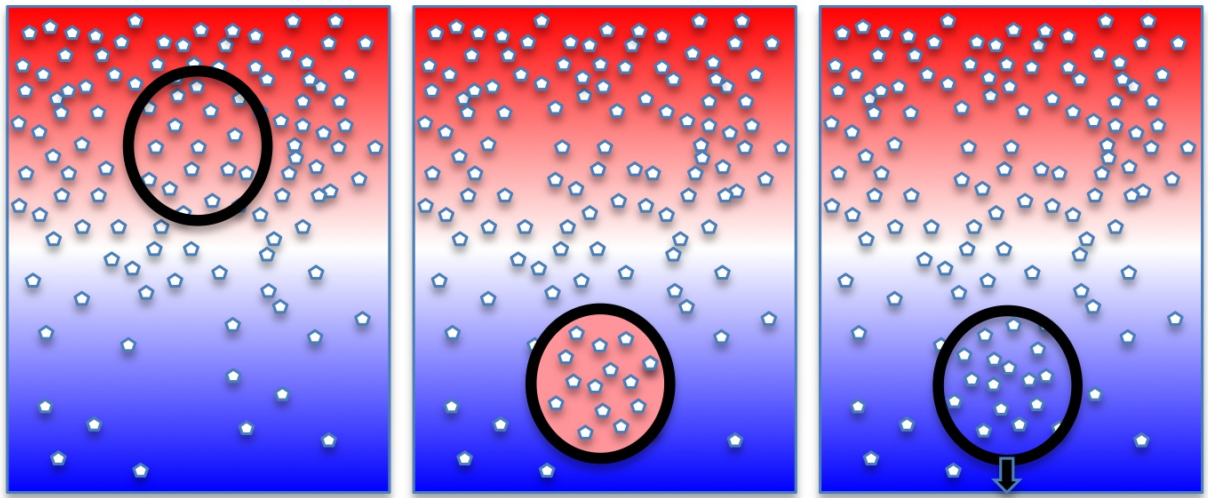
\includegraphics[width=.9\textwidth]{fingdiagram.png}\footnote{\citep{Garaud2014}}
% 		\label{fig:figs_scdiagram}
% 		\caption{Fingering (FC; also Thermohaline, Thermocompositional) Convection}
% 	\end{figure}}
% 	\only<2>{
% 	\begin{figure}[h]
% 		\centering
% 			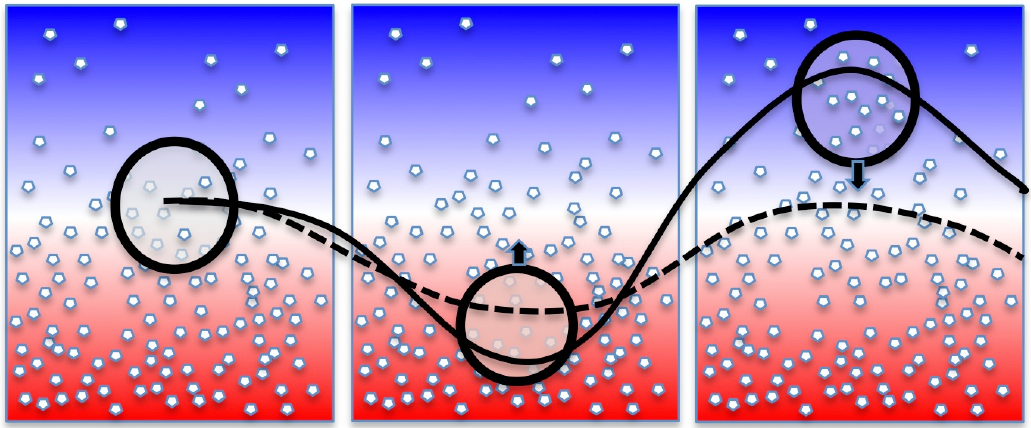
\includegraphics[width=.9\textwidth]{scdiagram.png}\footnote{\citep{Garaud2014}}
% 		\label{fig:figs_scdiagram}
% 		\caption{Oscillatory Double-Diffusive Convection (ODDC; also sometimes Semi-Convection)}
% 	\end{figure}}
% \end{overprint}
% }

% \frame{\frametitle{Double-diffusive convection occurs in several physical scenarios.}
% \begin{itemize}
% 	\item FC
% 	\begin{itemize}
% 		\item Thermocline of the ocean
% 		\item Red Giant Branch of Sun-like stars
% 	\end{itemize}
% 	\item ODDC
% 	\begin{itemize}
% 		\item Beneath the arctic ice cap (also intrusions)
% 		\item Throughout massive star evolution
% 	\end{itemize}
% \end{itemize}
% In this talk (because I'm an astrophysics student), I will focus on the massive star applications.
% }

% \subsection{ODDC in Massive Stars}

% \frame{\frametitle{Massive stars ($>8M_\odot$) are significant because they produce a large fraction of the heavy elements either during their evolution or in supernovae.}
% \begin{figure}[h]
% 	\centering
% 		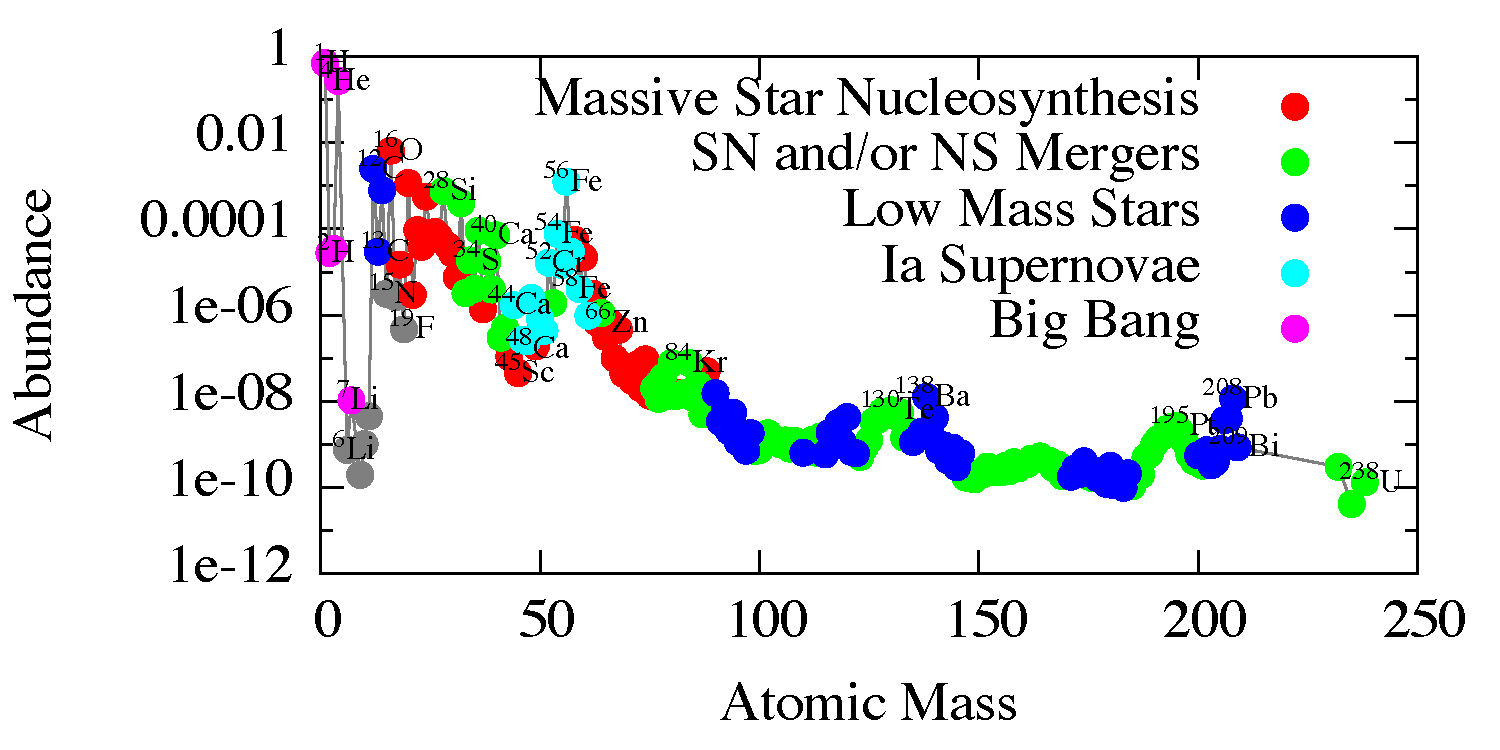
\includegraphics[width=.9\textwidth]{figs/abundances.pdf}\footnote{\citep{Lodders2010,Woosley2002,Burbidge1957}}
% 	\label{fig:figs_abundances}
% \end{figure}
% }

% \frame{\frametitle{ODDC is modeled in stars using the \citet{Langer1983} prescription by deriving a diffusion coefficient, $D$.}
% \begin{columns}
% 	\column{150pt}
% 	{\bf MESA \citep{Langer1983}}
% 	\begin{itemize}
% 		\item Only mixes composition
% 		\item One free parameter, $\alpha$
% 	\end{itemize}
% 	\begin{align}
% 		D=&\frac{\alpha \kappa_{T}}{6}\frac{\frac{dT}{dz}-\left.\frac{\partial T}{\partial z}\right|_{\rm{ad}}}{\frac{\phi T}{\delta \mu}\frac{d\mu}{dz}+\left.\frac{\partial T}{\partial z}\right|_{\rm{ad}}-\frac{dT}{dz}} \\
% 		\delta\equiv&-\frac{\partial \ln\rho}{\partial\ln T}, \phi\equiv\frac{\partial\ln\rho}{\partial\ln\mu}
% 	\end{align}
% 	\column{150pt}
% 	{\bf KEPLER \citep{Woosley1988}}
% 	\begin{itemize}
% 		\item Only mixes composition
% 		\item One free parameter, $F$
% 	\end{itemize}
% 	\begin{equation}
% 		D=\frac{F\kappa_{T}D_{b}}{F\kappa_{T}+D_{b}}
% 	\end{equation}
% 	\begin{equation}
% 		D_{b}\propto\left(\frac{dT}{dz}-\left.\frac{\partial T}{\partial z}\right|_{\rm{ad}}\right)^{\frac{1}{2}}
% 	\end{equation}
% \end{columns}
% }

% \frame{\frametitle{In particular, ODDC has strong relevance to stellar evolution because stellar cores are hot and heavy \citep{Robertson1972}.}
% 	\begin{figure}[h]
% 			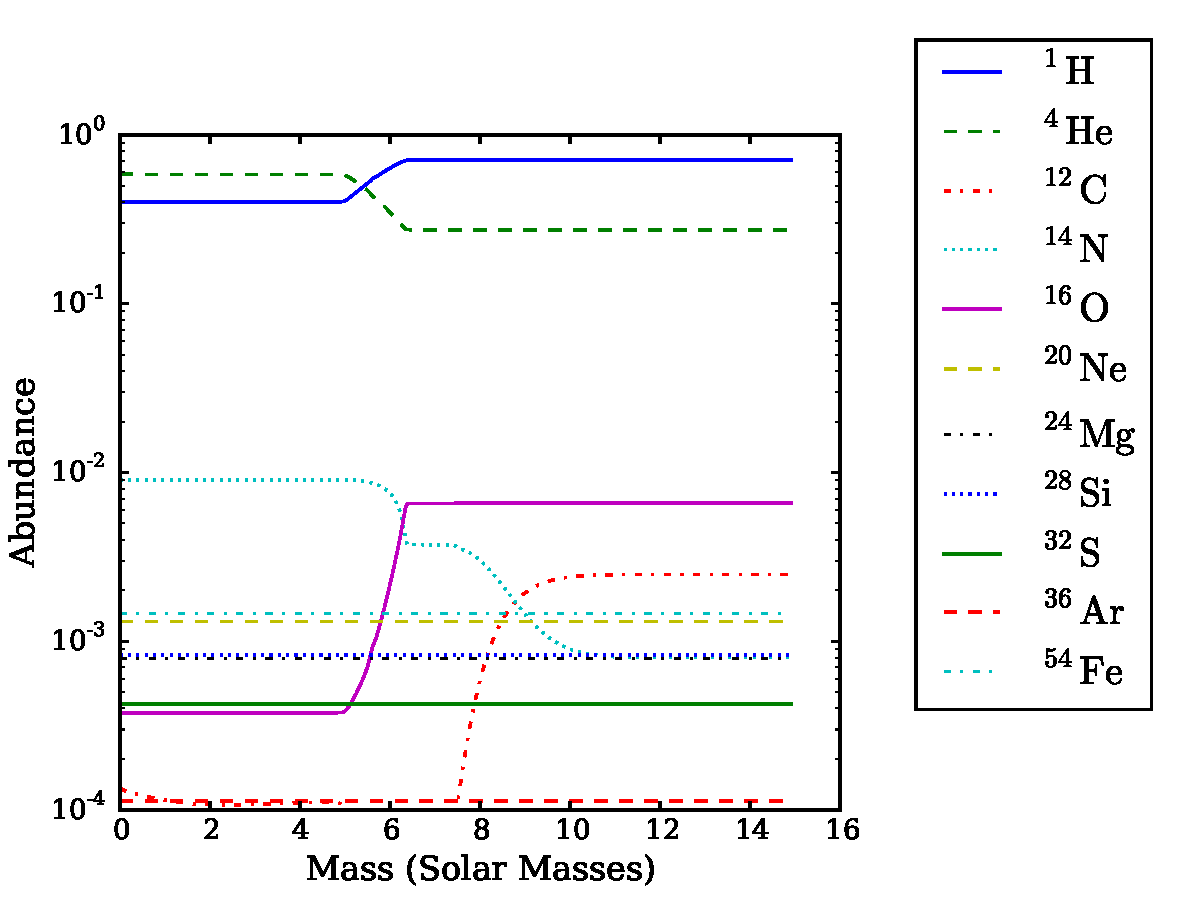
\includegraphics[width=.5\textwidth]{hburn_abun.pdf}
% 			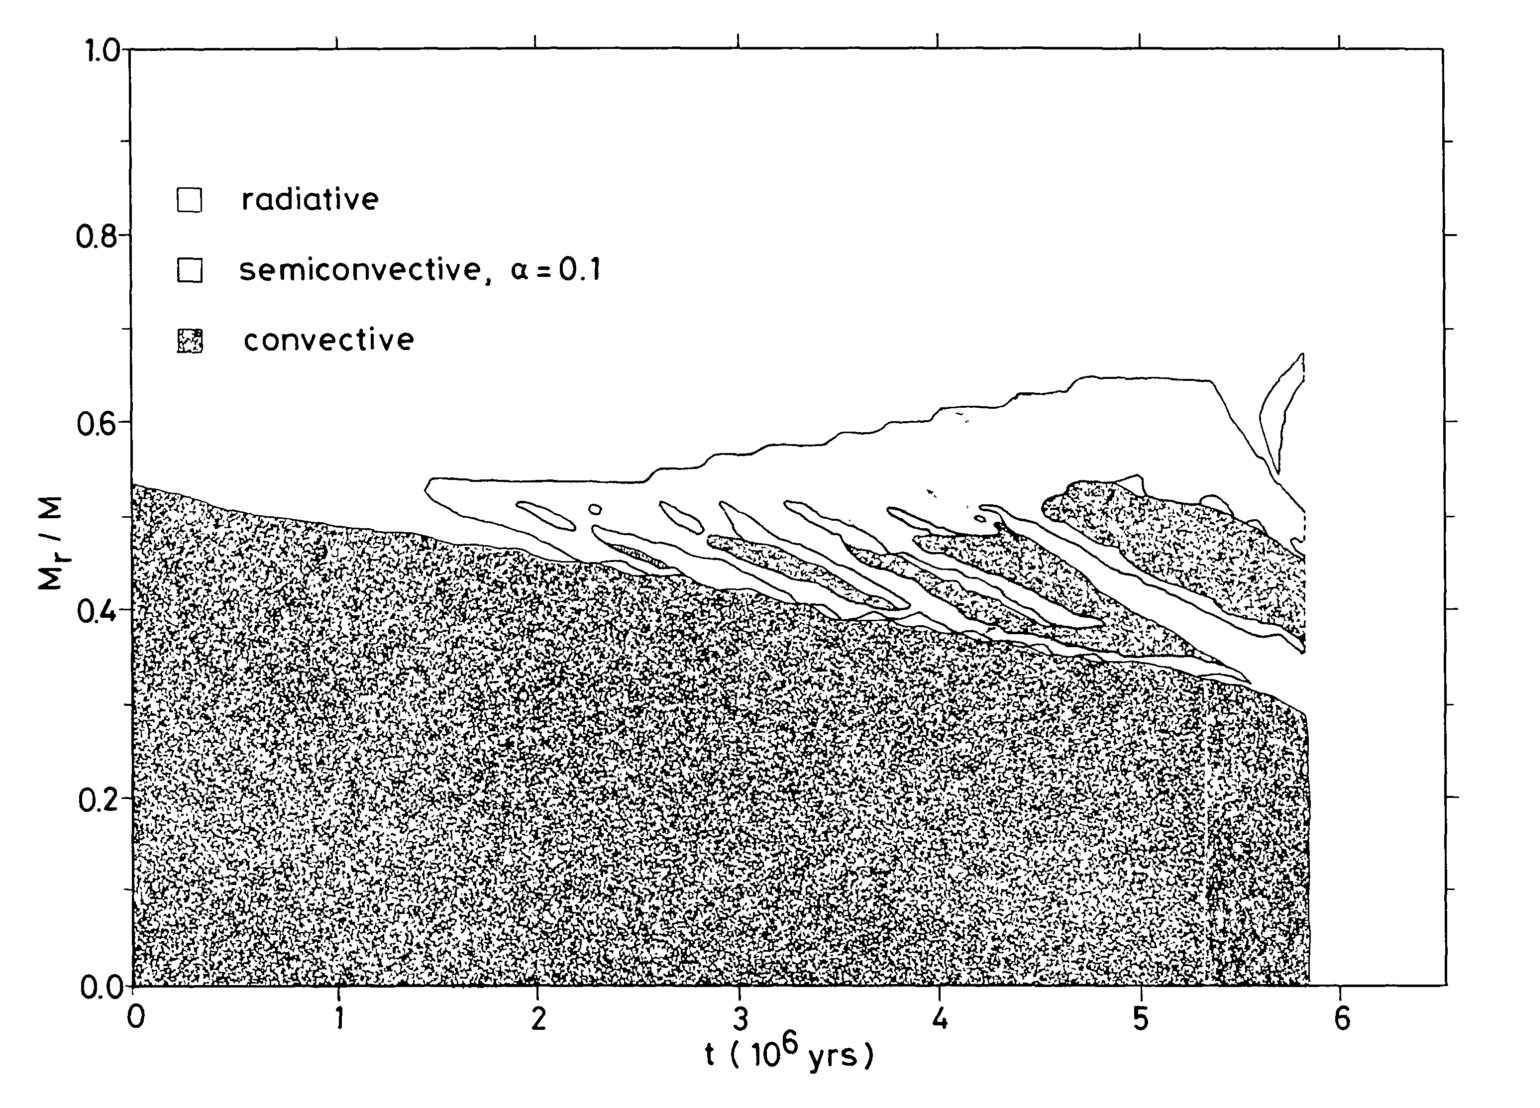
\includegraphics[width=.5\textwidth]{figs/Langer-core-sc.png}\footnote{\citep{Langer1985}}
% 		\label{fig:figs_Langer-core-sc}
% 	\end{figure}
% }
%
% \frame{\frametitle{The later stages of massive stars are complex.}
% \begin{figure}[h]
% 	\centering
% 		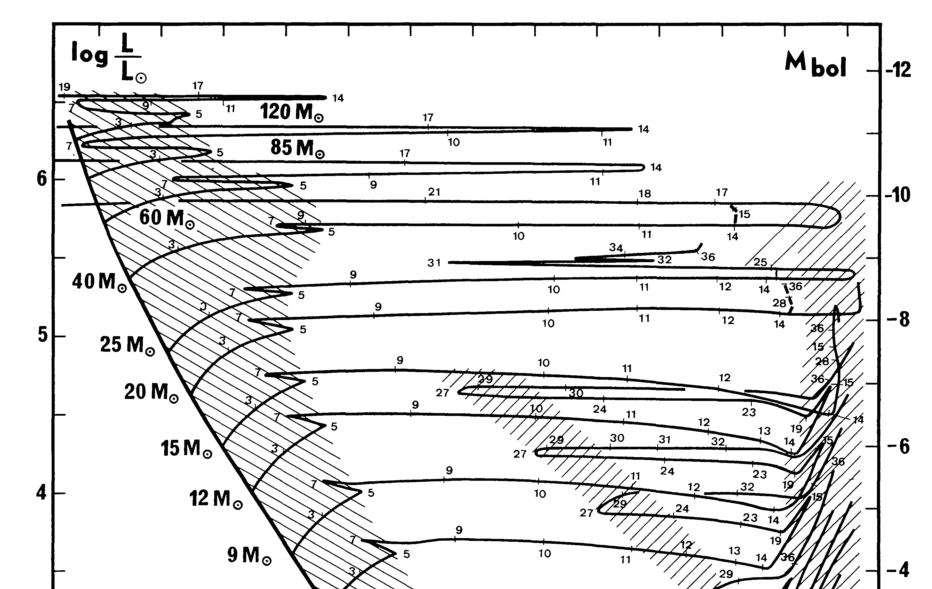
\includegraphics[width=.8\textwidth]{figs/Maeder-HR-head.png}
%
% 		\hspace{7pt}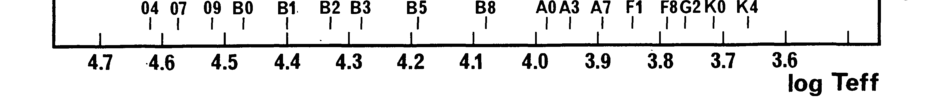
\includegraphics[width=.8\textwidth]{figs/Maeder-HR-foot.png}\footnote{\citep{Maeder1988}}
% 	\label{fig:figs_himasshr}
% \end{figure}
% }
%
% \frame{\frametitle{Since these late stages are dynamic, mixing processes (e.g. semi-convection) can drastically effect the final star structure and yields.}
% \begin{figure}[h]
% 	\centering
% 		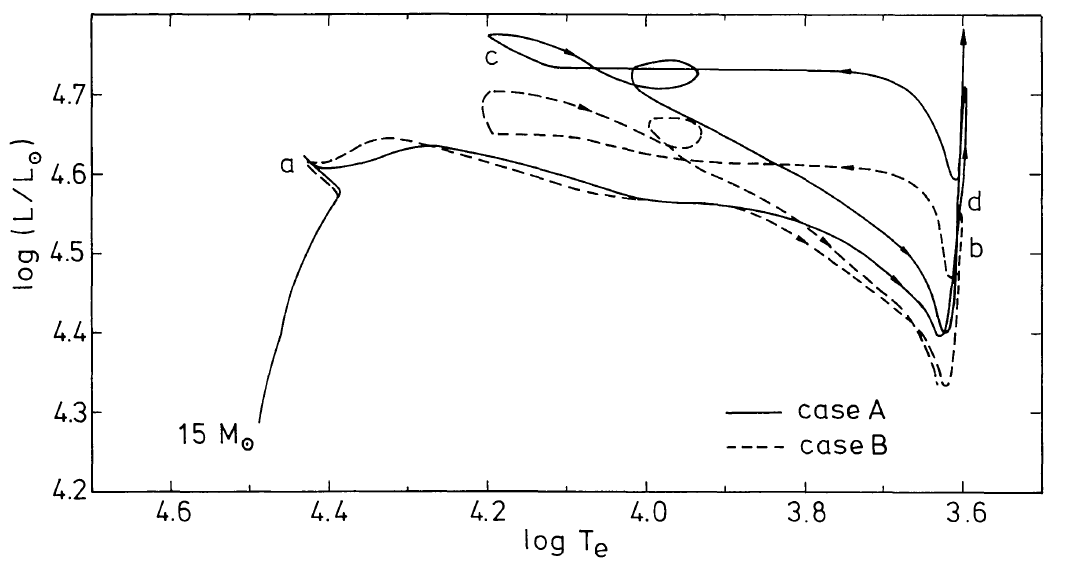
\includegraphics[width=.7\textwidth]{figs/semi_evolution.png}\footnote{\citep{Langer1985}}
% 		\caption{With semi-convection (solid), without (dashed)}
% 	\label{fig:figs_semi_evolution}
% \end{figure}
% }
%
% \frame{\frametitle{Small changes in the treatment of semi-convection can make the difference between stars becoming successful or failed supernovae by changing the final C/O cores.}
% \begin{figure}[h]
% 	\centering
% 		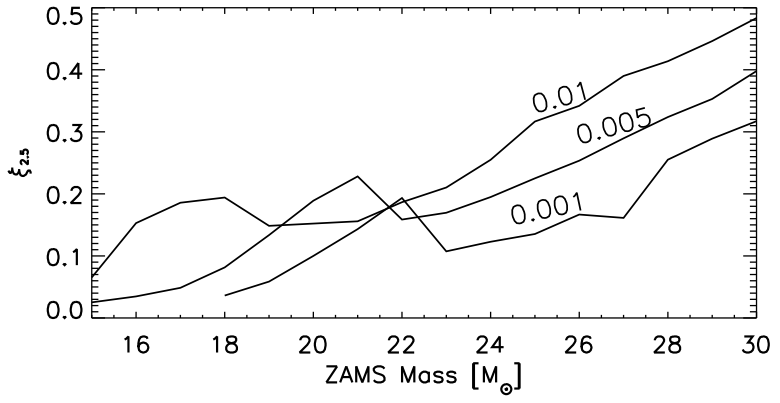
\includegraphics[width=.65\textwidth]{figs/compactness.png}\footnote{\citep{Sukhbold2014}}
% 		\caption{Likelihood of explosion, varying the semi-convection parameter from \citet{Woosley1988}}
% 	\label{fig:figs_compactness}
% \end{figure}
% }

\subsection{Overshooting Convection}

\frame{\frametitle{Overshooting convection is characterized by a convective region mixing into a nominally stable region.}
	\begin{figure}[h]
		\centering
			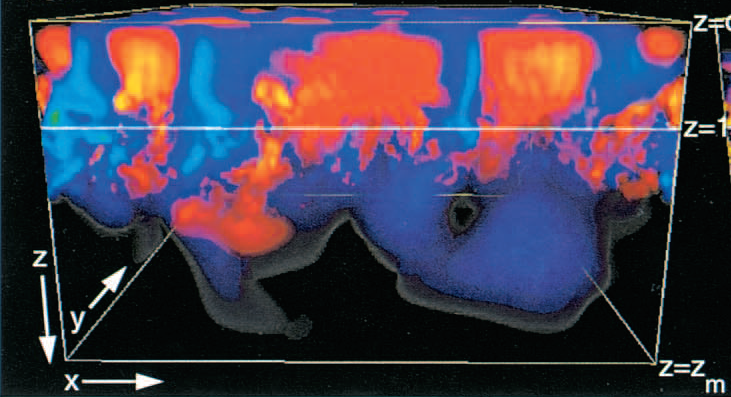
\includegraphics[width=.9\textwidth]{os_image.png}\footnote{\citep{Brummell2002}}
		\label{fig:figs_scdiagram}
	\end{figure}
}

\frame{\frametitle{This is distinct from penetrative convection, where the additional mixing extends the convection zone.}
	\begin{figure}[h]
		\centering
			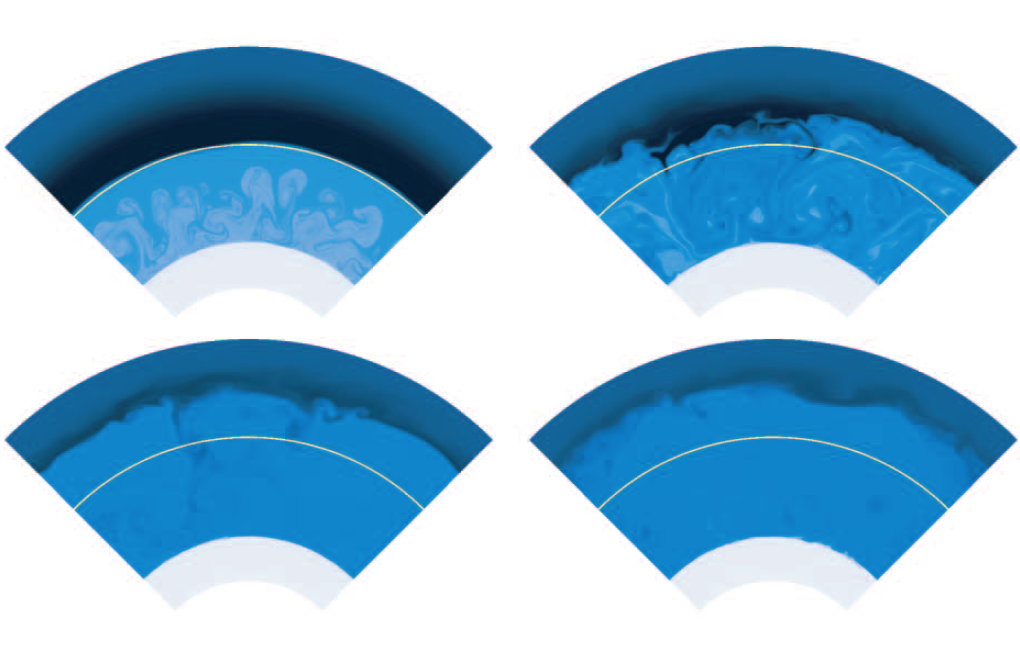
\includegraphics[width=.85\textwidth]{meakin_penetration.png}\footnote{\citep{Meakin2007}}
		\label{fig:figs_scdiagram}
	\end{figure}
}

\frame{\frametitle{Most numerical studies of overshooting convection investigate the effects of \textbf{stratification} at boundaries.}
	Some recent examples:
	\begin{itemize}
		\item \citet{Brummell2002}
		\item \citet{Meakin2007}
		\item \citet{Gilet2013}
	\end{itemize}
	Some convective boundaries are affected by varying \textbf{diffusion}, e.g. envelope convection and core helium burning.
}

\subsection{Setup}

\frame{\frametitle{Under the Boussinesq approximation, there are three possibilities for an overshooting region.}
	\begin{itemize}
		\item A spatially-dependent thermal expansion coefficient
		\item A spatially-dependent heating term
		\item A spatially-dependent diffusion coefficient
	\end{itemize}
}

\frame{\frametitle{Governing equations \citep{Spiegel1960}}
\begin{overprint}
\only<1>{
Assuming the Boussinesq approximation and an adiabatic temperature gradient (such as appears during a formal derivation of the Boussinesq approximation for a gas) yields
\begin{align}
	\rho_{0}\frac{D}{D{t}}{\mathbf{u}} =& -\nabla p + \rho_{0}\alpha g T + \rho_{0}\nu\nabla^{2}\mathbf{u} \\
	\nabla\cdot\mathbf{u} =& 0 \\
	\rho_{0}\frac{D}{D{t}}{T} - \rho_{0}\left.\frac{d}{dz}T\right|_{\mathrm{ad}} =& \rho_{0}\nabla^{2}\kappa_{T}(z) T + H\left(z\right) \\
\end{align}
for the case with uniform diffusion but a z-dependent heating term.}
\only<2>{
or
\begin{align}
	\rho_{0}\frac{D}{D{t}}{\mathbf{u}} =& -\nabla p + \rho_{0}\alpha g T + \rho_{0}\nu\nabla^{2}\mathbf{u} \\
	\nabla\cdot\mathbf{u} =& 0 \\
	\rho_{0}\frac{D}{D{t}}{T} - \rho_{0}\left.\frac{d}{dz}T\right|_{\mathrm{ad}} =& \rho_{0}\nabla\cdot \left(\kappa_{T,0}+\kappa_{T}(z)\right)\nabla T \\
\end{align}
for the case with nonuniform diffusion.}
\only<3>{
Subtracting a static background temperature and non-dimensionalizing yields
\begin{align}
	\frac{D}{D{t}}{\mathbf{u}} =& -\nabla p + \frac{\mathrm{Ra}_{T}}{\mathrm{Pr}}{T} + \nabla^{2}\mathbf{u} \\
	\nabla\cdot\mathbf{u} =& 0 \\
	\frac{D}{D{t}}{T} + w f\left(z\right) =& \nabla\cdot \left(\mathrm{Pr}+\kappa_{T}(z)/\kappa_{T,0}\right)^{-1}\nabla T, \\
\end{align}
where $\kappa_{T}(z)$ is zero in the uniform diffusion case.}
\end{overprint}
% \begin{overprint}
% \only<1>{
% \begin{align}
% 	\rho_{0}\frac{D}{D{t}}{\mathbf{u}} =& -\nabla p + \left(-\alpha{T}+\beta\mu\right)\rho_{0}\mathbf{g} + \nu\rho_{0}\nabla^{2}\mathbf{u} \\
% 	\nabla\cdot\mathbf{u} =& 0 \\
% 	\frac{D}{D{t}}{T} + w\frac{d}{dz}T_{0} =& \kappa_T \nabla^{2}T \\
% 	\frac{D}{D{t}}{\mu} + w\frac{d}{dz}\mu_{0}=& \kappa_{\mu}\nabla^{2}\mu
% \end{align}}
% \only<2>{
% \begin{align}
% 	\frac{1}{\rm{Pr}}\frac{D}{D{t}}{\mathbf{u}} =& -\nabla p + \left(-T+\mu\right)\mathbf{\hat{z}} + \nabla^{2}\mathbf{u},\rm{Pr}\equiv\frac{\nu}{\kappa_{T}} \\
% 	\nabla\cdot\mathbf{u} =& 0 \\
% 	\frac{D}{D{t}}{T} \pm w =& \nabla^{2}T \\
% 	\frac{D}{D{t}}{\mu} \pm \frac{w}{R_{0}}=& \tau\nabla^{2}\mu, R_{0}\equiv\frac{\alpha\left(T_{0z}-T_{\rm{ad},z}\right)}{\beta\mu_{0z}}, \tau\equiv\frac{\kappa_{\mu}}{\kappa_{T}}
% \end{align}
% The $+$ corresponds to FC and the $-$, ODDC.}
% \end{overprint}
}

% \frame{\frametitle{Depending on the strength of the stabilizing composition, semi-convection can be in various forms.}
% \begin{overprint}
% 	\only<1>{
% 	\begin{equation}
% 		1<R_{0}^{-1}<\frac{\rm{Pr} + 1}{\rm{Pr} + \tau}
% 	\end{equation}
% 	\vspace{-100pt}
% 	\begin{figure}[h]
% 		\centering
% 			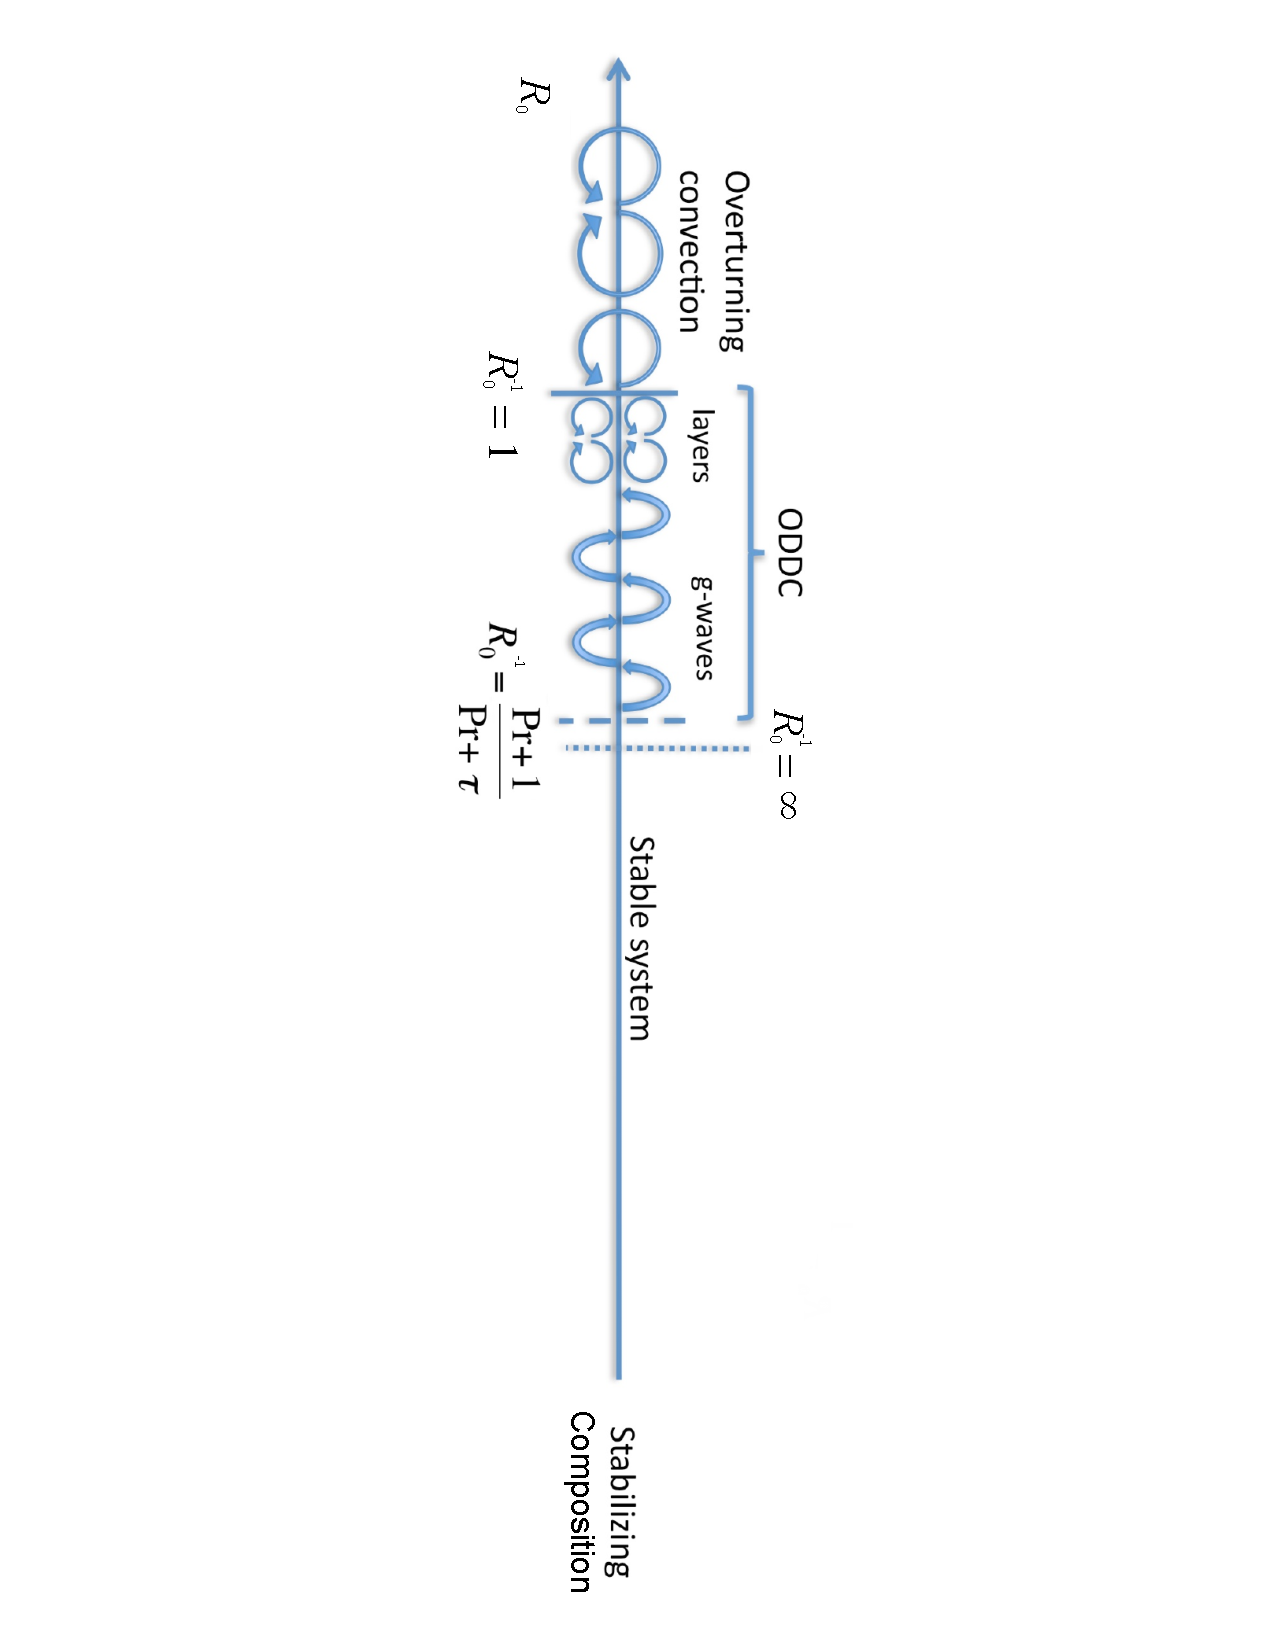
\includegraphics[width=.8\textwidth,angle=90]{../pngs/regimes-sc-flip-1.pdf}\footnote{\citep{Garaud2014}}
% 		\label{fig:pngs_regimes}
% 	\end{figure}
% 	\vspace{-100pt}
% 	}
% 	\only<2>{
% 	\begin{figure}[h]
% 		\centering
% 			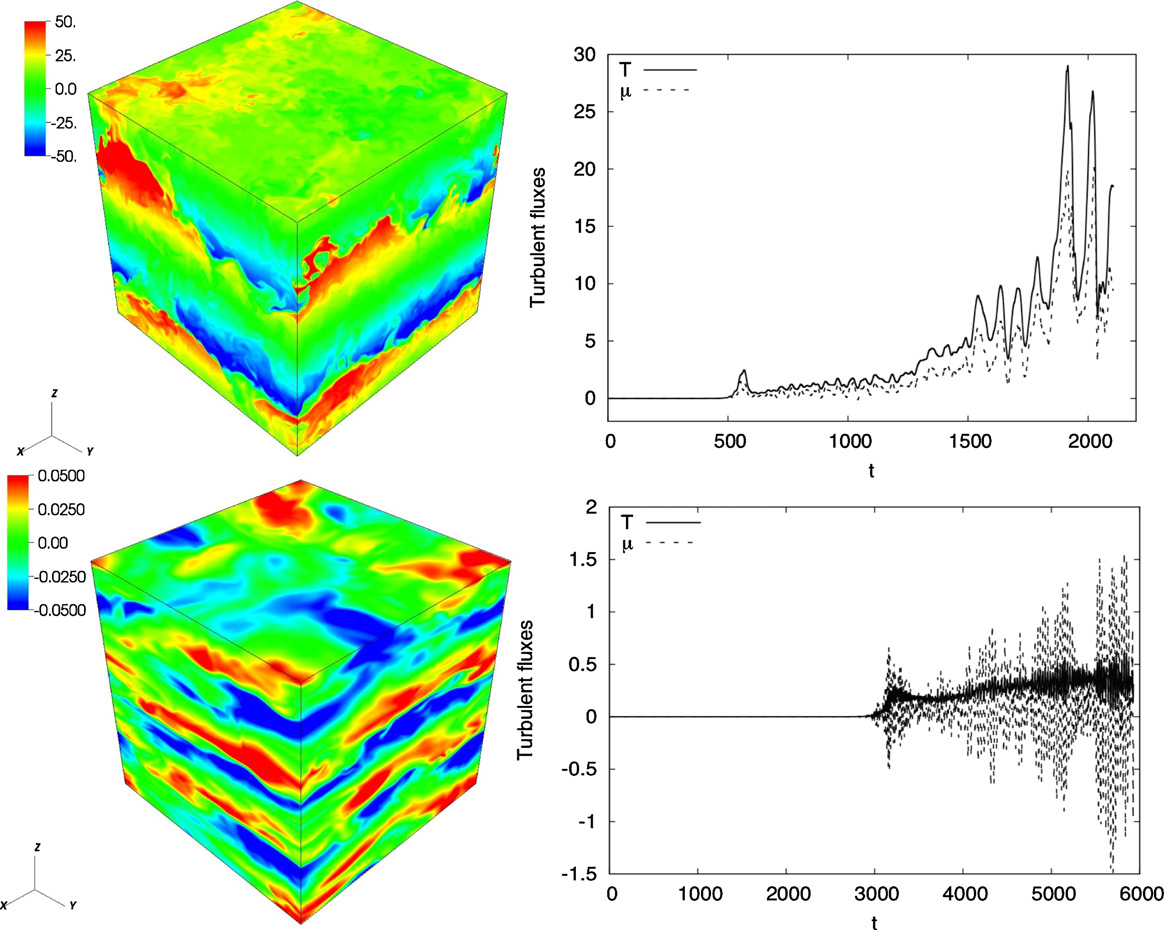
\includegraphics[width=.5\textwidth]{../pngs/regimes_image.png}\footnote{\citep{Mirouh2012}}
% 			\caption{$\rm{Pr}=\tau=0.03$, $R_{0}^{-1}=1.5\mbox{ (top)},5.0\mbox{ (bottom)}$}
% 		\label{fig:pngs_regimes_image}
% 	\end{figure}
% 	}
% \end{overprint}
% }

% \frame{\frametitle{To determine which regime is relevant to stars, we look at the condition for layer formation from \citet{Mirouh2012}.}
% 	\begin{figure}[h]
% 		\centering
% 			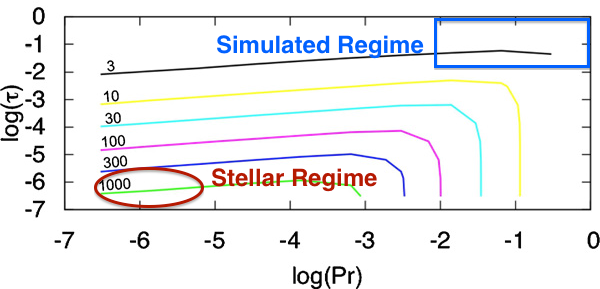
\includegraphics[width=0.9\textwidth]{../pngs/layer_condition.png}\footnote{\citep{Mirouh2012}}
% 			\caption{$R_{L}^{-1}$, the maximum $R_{0}^{-1}$ for which layers exist}
% 		\label{fig:pngs_layer_condition}
% 	\end{figure}
% }

% \frame{\frametitle{We find in KEPLER simulations that semi-convection regions exist preferentially in the layer-forming regime.}
% \begin{figure}[h]
% 	\centering
% 		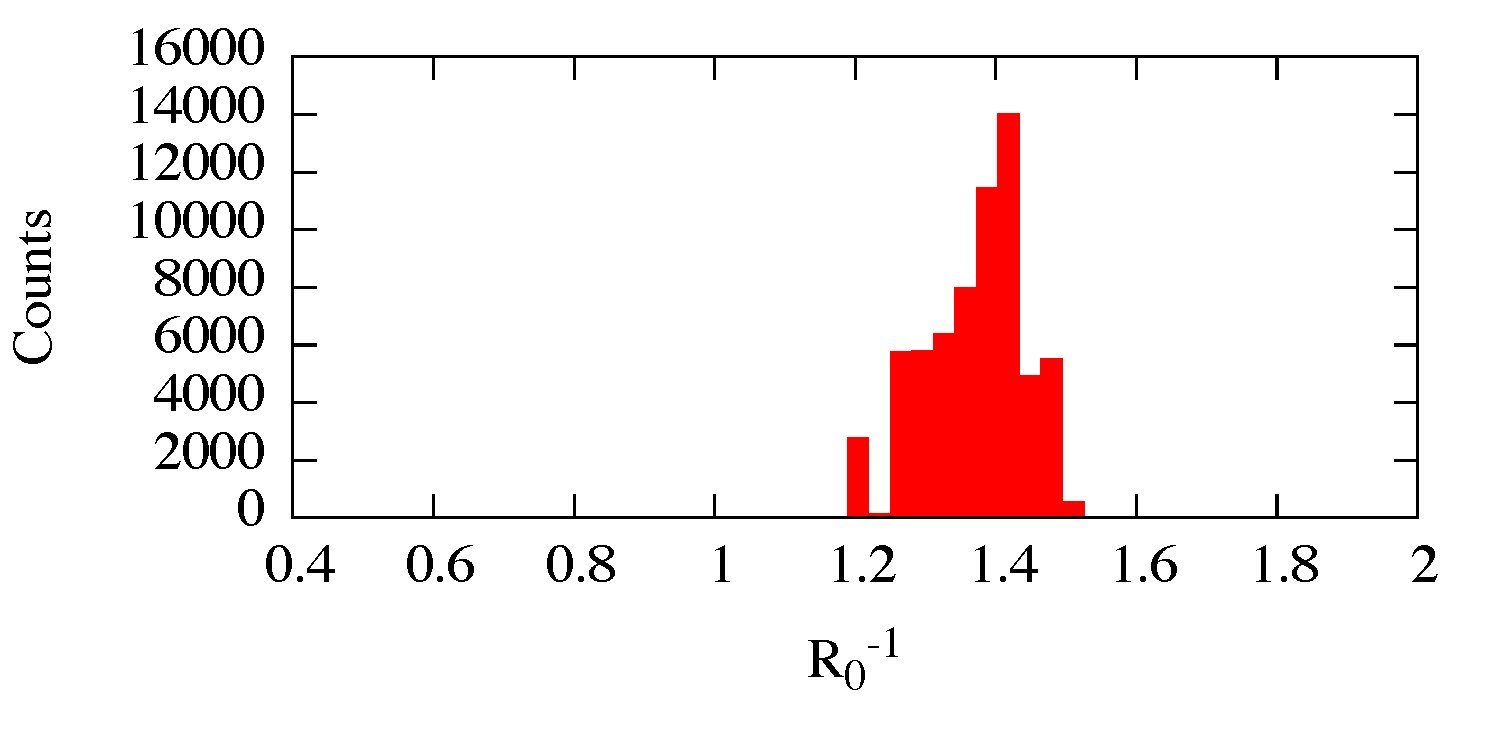
\includegraphics[width=.9\textwidth]{figs/r0hist.pdf}
% 	\caption{For semi-convection to be in the layered regime, $1<R_{0}^{-1}<R_{L}^{-1}\sim1000$} 
% 	\label{fig:figs_r0hist}
% \end{figure}
% }

% \subsection{Model}

% \frame{\frametitle{\citet{Wood2013} determined an empirical model for the fluxes in layers with one free parameter, $l_{\rm{semi}}$.}
% 	\begin{figure}[h]
% 		\centering
% 			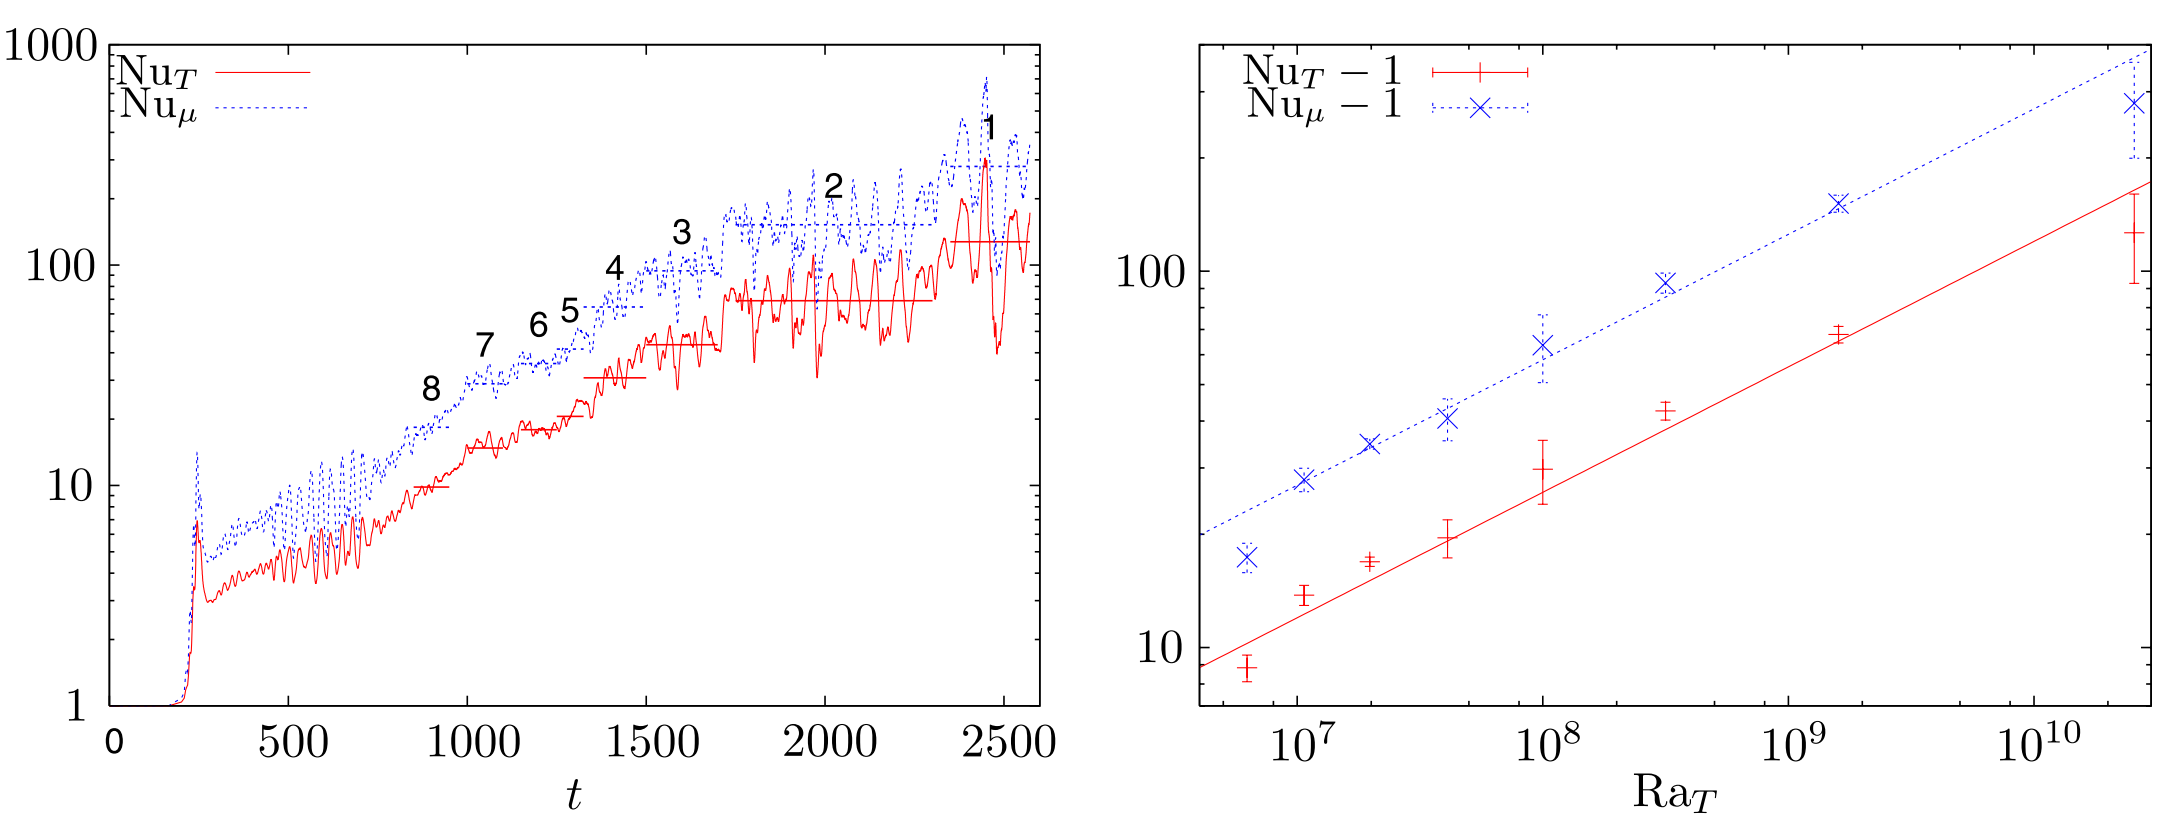
\includegraphics[width=.9\textwidth]{figs/wood-layers.png}\footnote{\citep{Wood2013}}
% 		\label{fig:figs_wood-layers}
% 	\end{figure}
% \begin{overprint}
% 	\only<1>{\begin{equation}
% Q_{\rm{semi}}=-0.1\left(\frac{g\delta|\frac{dT}{dr}-\left.\frac{dT}{dr}\right|_{\rm ad}|(l_{\rm semi})^{4}}{T\kappa_{T}^{2}}\right)^{1/3}\rho{c_{p}}\kappa_{T}\left(\frac{dT}{dr}-\left.\frac{dT}{dr}\right|_{\rm ad}\right)
% \end{equation}}
% \only<2>{\begin{equation}
% 		\kappa_{\mu, {\rm semi}}=0.03\left(\nu\kappa_{T}^{3}\right)^{1/4}\left(\frac{g\delta|\frac{dT}{dz}-\left.\frac{dT}{dz}\right|_{\rm ad}|(l_{\rm semi})^{4}}{\nu T\kappa_{T}}\right)^{0.37}
% 	\end{equation}}
% \end{overprint}
% }

% \frame{\frametitle{The Boussinesq approximation does not constrain the layer height; layers merge until they fill the domain.}
% \begin{figure}[h]
% 	\centering
% 		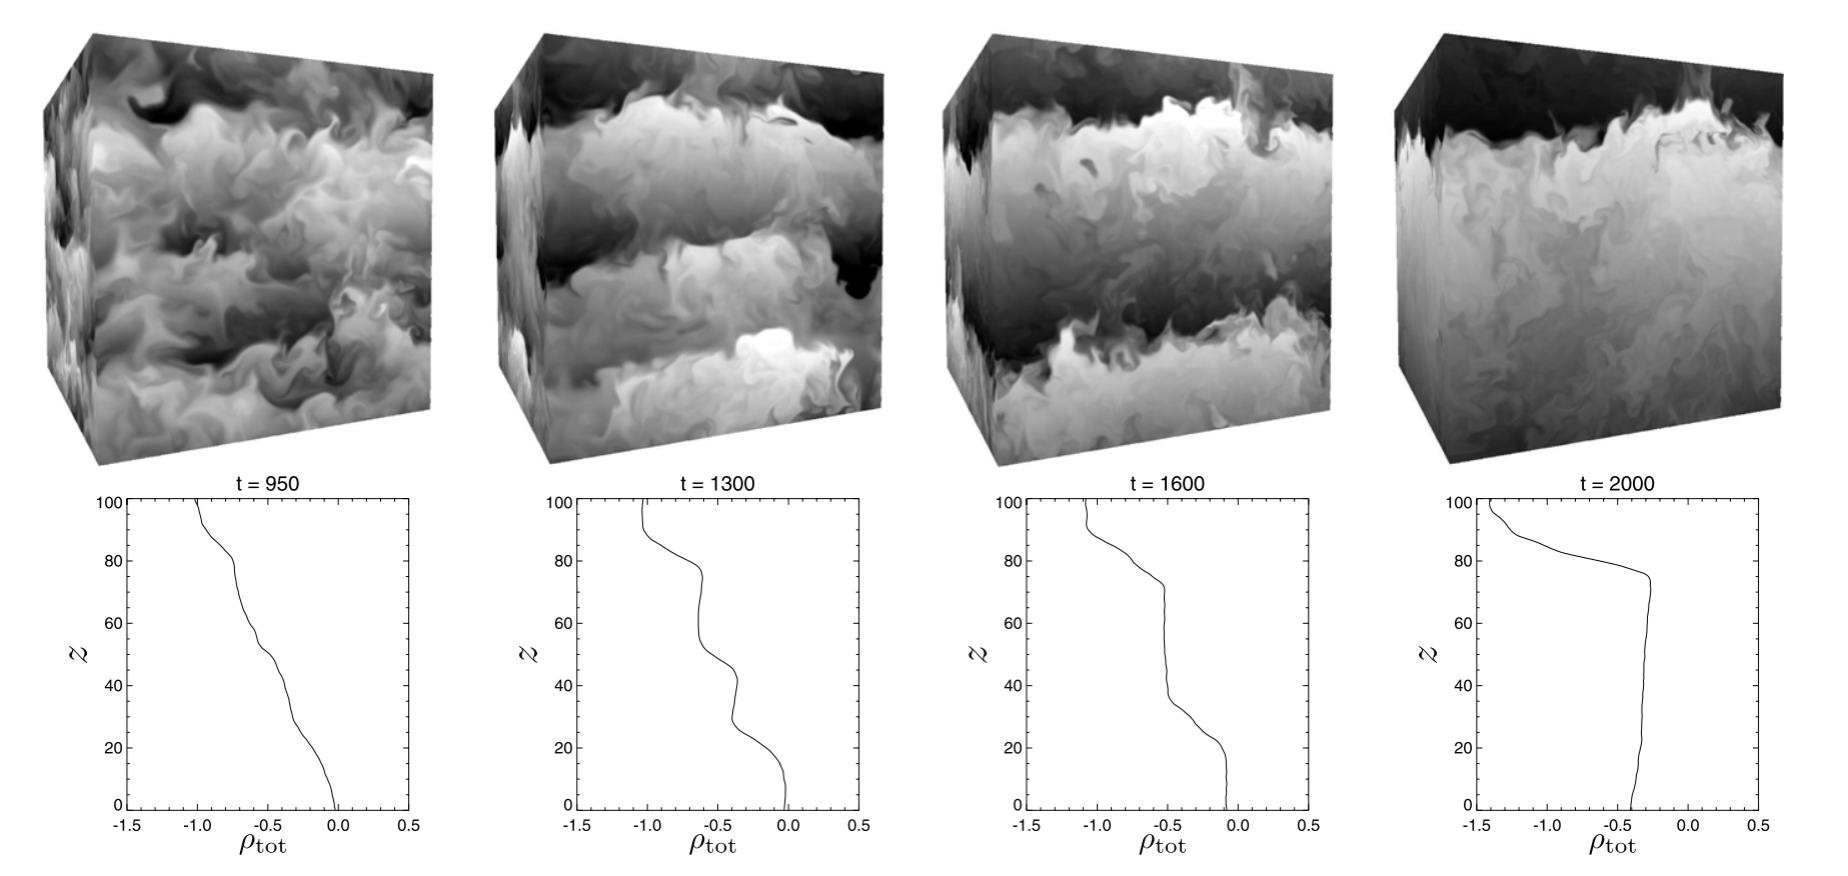
\includegraphics[width=.9\textwidth]{figs/layer-merge.png}\footnote{\citep{Wood2013}}
% 	\label{fig:figs_layer-merge}
% \end{figure}
% }

% \frame{\frametitle{We'd like to perform a new series of simulations to determine the maximum height of these layers.}
% \begin{itemize}
% 	\item Cover new physics not present in PADDI
% 	\begin{itemize}
% 		\item Non-linear diffusion
% 		\item Pseudo-incompressibility 
% 	\end{itemize}
% 	\item Attempt larger domains
% 	\begin{itemize}
% 		\item Move to 2D for this to be feasible
% 	\end{itemize}
% 	\item Finely resolve only layer interfaces
% 	\begin{itemize}
% 		\item Not possible in a traditional spectral code!
% 	\end{itemize}
% \end{itemize}
% }

\frame{\frametitle{A simple solution to this is a spectral element code using Chebyshev polynomials in the vertical direction.}
\begin{columns}
	\column{125pt}
	\begin{itemize}
		\item Solves by Chebyshev collocation
		\begin{itemize}
			\item Trivial to solve space-dependent diffusion
			\item Fine resolution at element boundaries
			\item Coarse resolution at element centers  
		\end{itemize}
	\end{itemize}
	\column{175pt}
	\begin{figure}[h]
		\centering
			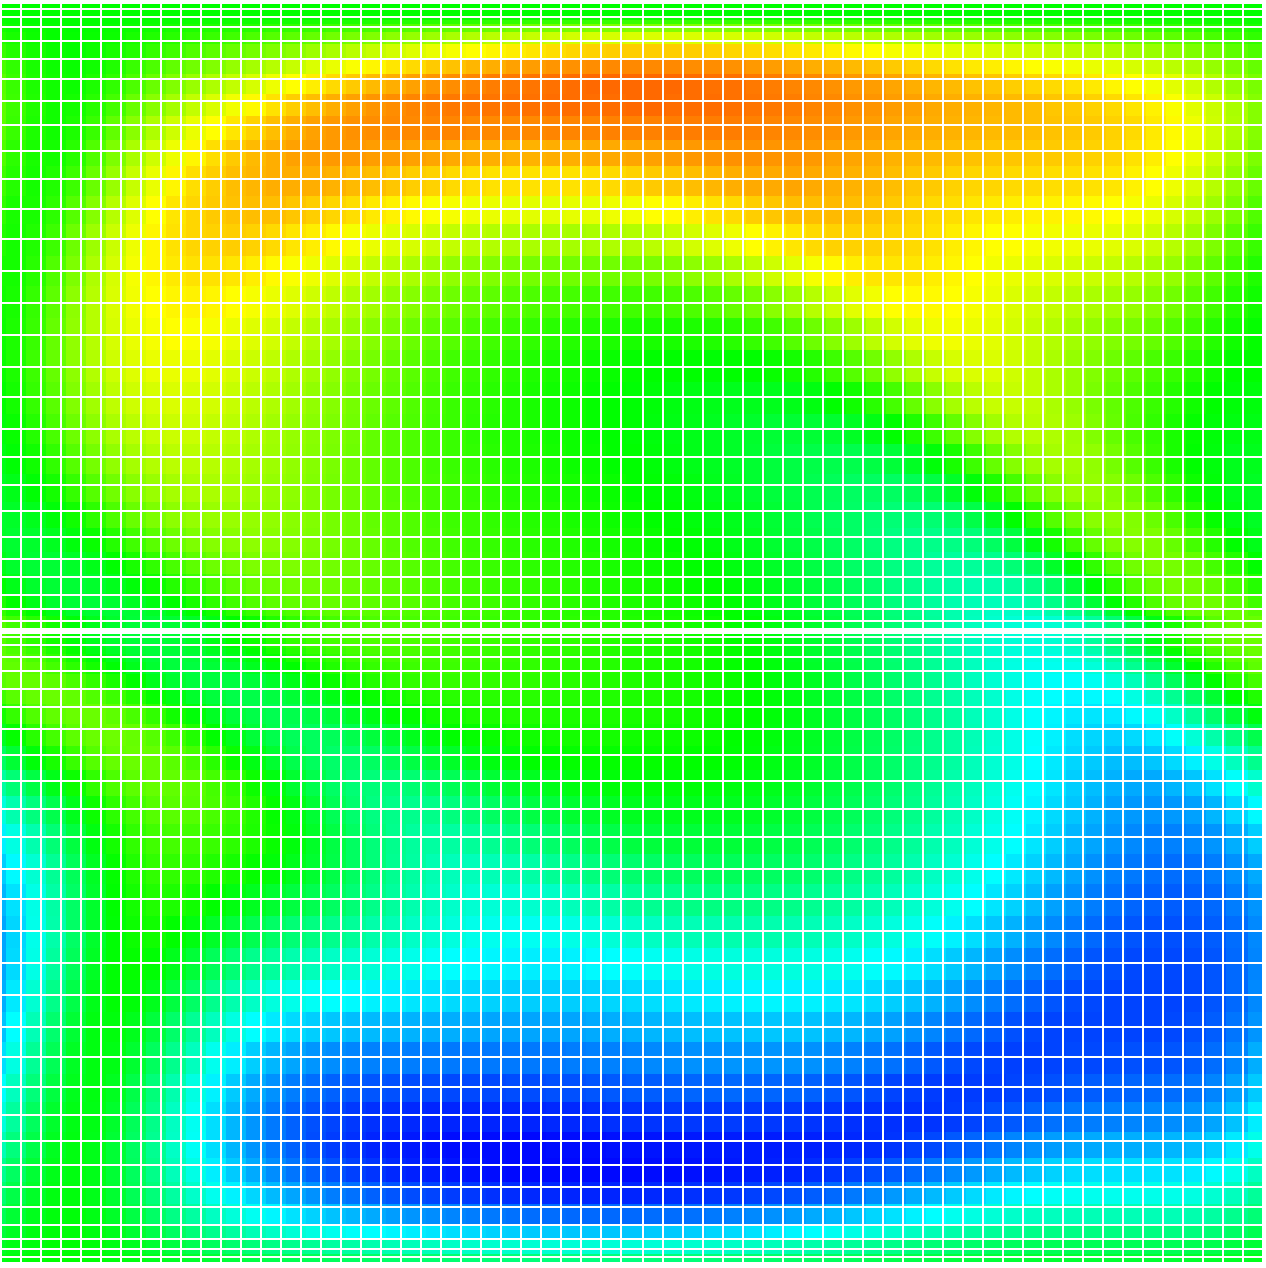
\includegraphics[width=.9\textwidth]{figs/grid.png}
		\label{fig:figs_grid}
	\end{figure}
\end{columns}
}

% \frame{\frametitle{We've run simulations in 2D and 3D with PADDI, and find similar results---except in particular cases with strong shear.}
% \setbeamercovered{transparent}
% \begin{tabular}{r c c}
% 	\vtop{\null\hbox{\scalebox{0.7}{\begin{tabular}{r}
% 		$\rm{Pr}=0.03$ \\
% 		$\tau=0.3$ \\
% 		$R_{0}^{-1}=1.1,1.2$ \\
% 	\end{tabular}}}} &
% 	\fbox{\vtop{\null\hbox{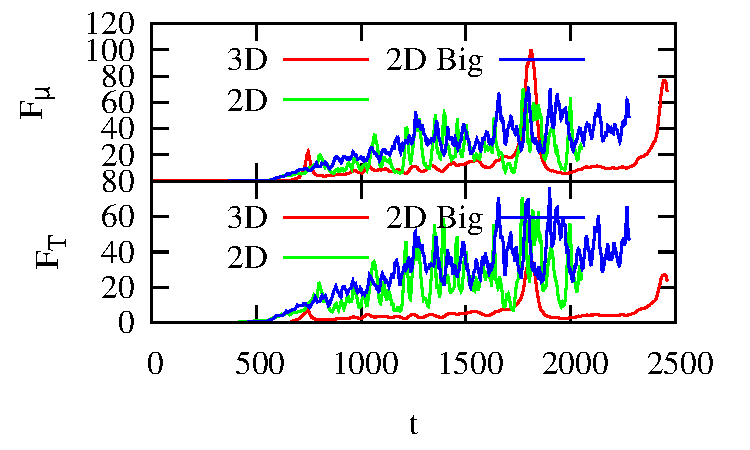
\includegraphics[width=0.35\textwidth]{figs/Pr=0_03_t=0_3_R0-1=1_1.pdf}}}} &
% 	\fbox{\vtop{\null\hbox{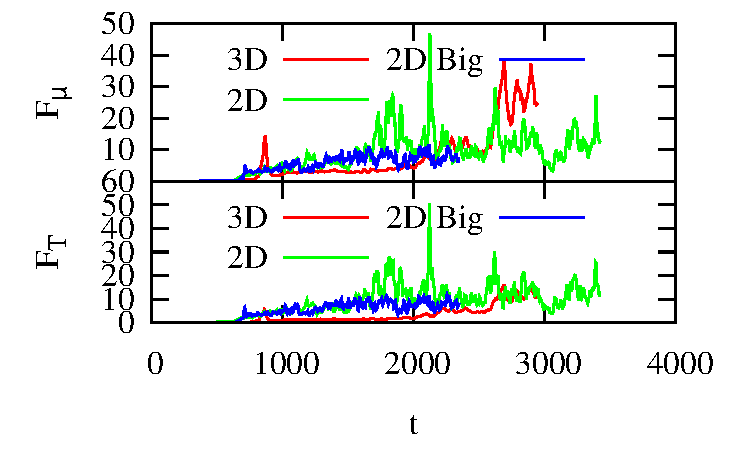
\includegraphics[width=0.35\textwidth]{figs/Pr=0_03_t=0_3_R0-1=1_2.pdf}}}} \\
% 	\vtop{\null\hbox{\scalebox{0.7}{\begin{tabular}{r}
% 		$\rm{Pr}=0.01$ \\
% 		$\tau=0.01$ \\
% 		$R_{0}^{-1}=1.5,2$ \\
% 	\end{tabular}}}} &
% 	\vtop{\null\hbox{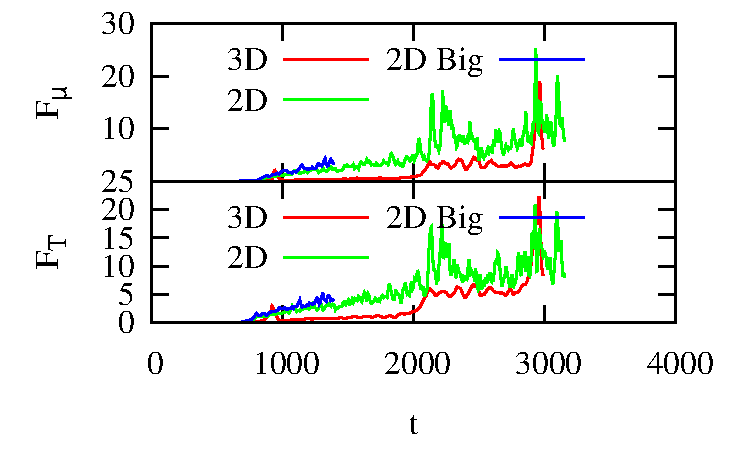
\includegraphics[width=0.35\textwidth]{figs/Pr=0_01_t=0_01_R0-1=1_5.pdf}}} &
% 	\vtop{\null\hbox{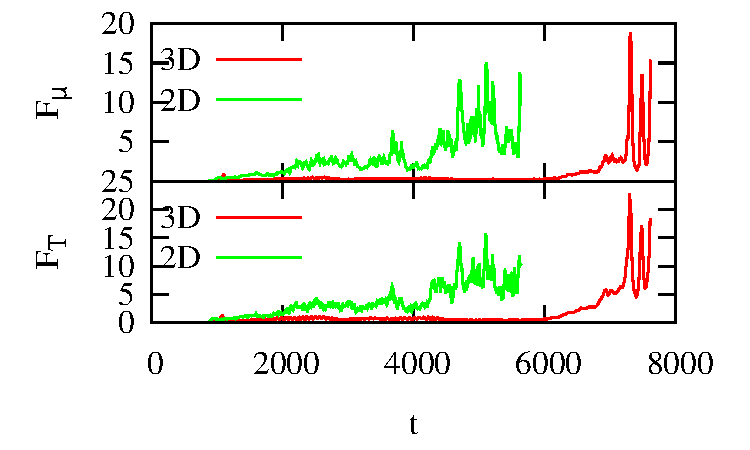
\includegraphics[width=0.35\textwidth]{figs/Pr=0_01_t=0_01_R0-1=2.pdf}}} \\
% \end{tabular}
% }

% \frame{\frametitle{At early stages, the simulations have similar behavior; however, at late stages, large shear dominates the 2D runs.}
% \begin{overprint}
% 	\only<1>{
% 	\begin{figure}[h]
% 		\centering
% 			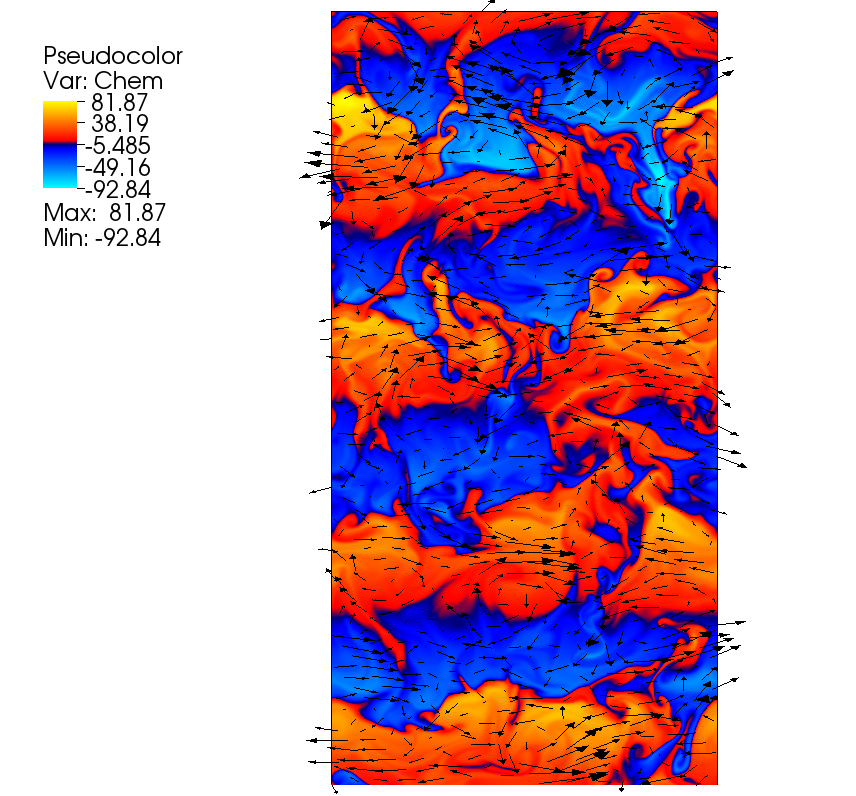
\includegraphics[width=.55\textwidth]{../pngs/movie0003.png}
% 		\label{fig:pngs_movie0003}
% 		\caption{$\rm{Pr}=0.3$, $\tau=0.3$, $R_{0}^{-1}=1.15$}
% 	\end{figure}
% 	}
% 	\only<2>{
% 	\begin{figure}[h]
% 		\centering
% 			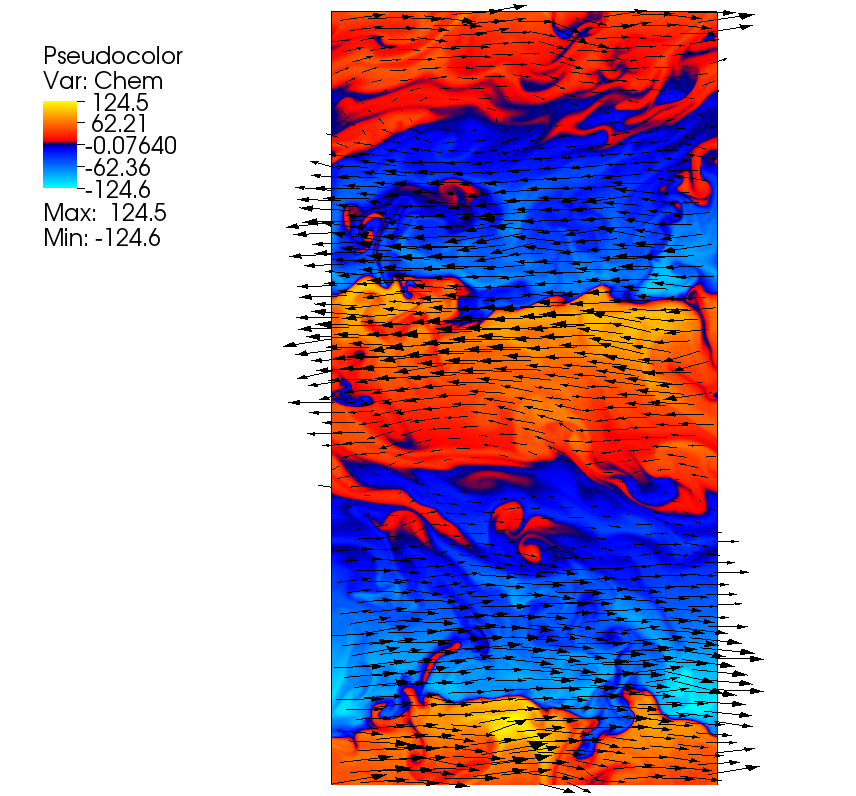
\includegraphics[width=.55\textwidth]{../pngs/movie0014.png}
% 		\label{fig:pngs_movie0014}
% 		\caption{$\rm{Pr}=0.3$, $\tau=0.3$, $R_{0}^{-1}=1.15$}
% 	\end{figure}
% 	}
% \end{overprint}
% }

% \frame{\frametitle{Fortunately, this problem appears absent in the low viscosity and compositional diffusivity runs at low $R_0^{-1}$.}
% \setbeamercovered{transparent}
% \begin{tabular}{r c c}
% 	\vtop{\null\hbox{\scalebox{0.7}{\begin{tabular}{r}
% 		$\rm{Pr}=0.03$ \\
% 		$\tau=0.3$ \\
% 		$R_{0}^{-1}=1.1,1.2$ \\
% 	\end{tabular}}}} &
% 	\vtop{\null\hbox{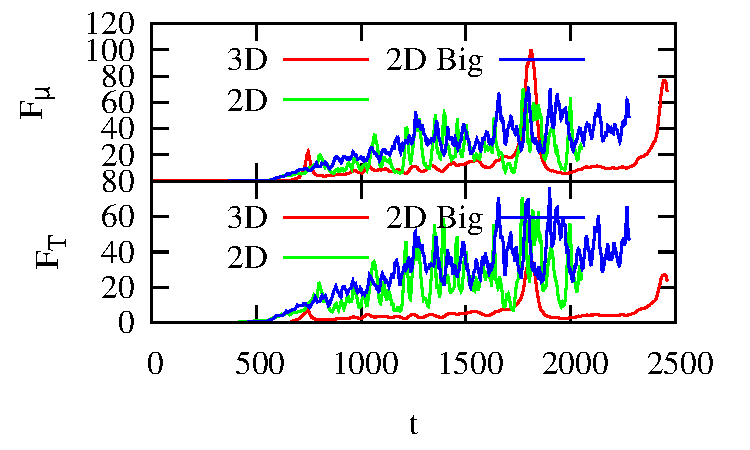
\includegraphics[width=0.35\textwidth]{figs/Pr=0_03_t=0_3_R0-1=1_1.pdf}}} &
% 	\vtop{\null\hbox{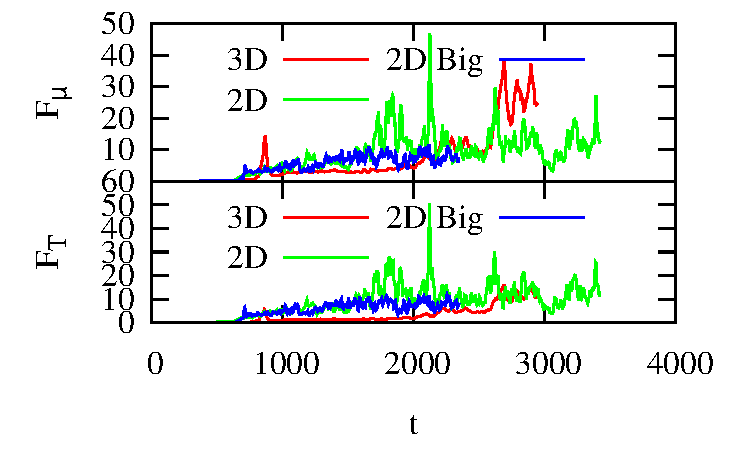
\includegraphics[width=0.35\textwidth]{figs/Pr=0_03_t=0_3_R0-1=1_2.pdf}}} \\
% 	\vtop{\null\hbox{\scalebox{0.7}{\begin{tabular}{r}
% 		$\rm{Pr}=0.01$ \\
% 		$\tau=0.01$ \\
% 		$R_{0}^{-1}=1.5,2$ \\
% 	\end{tabular}}}} &
% 	\fbox{\vtop{\null\hbox{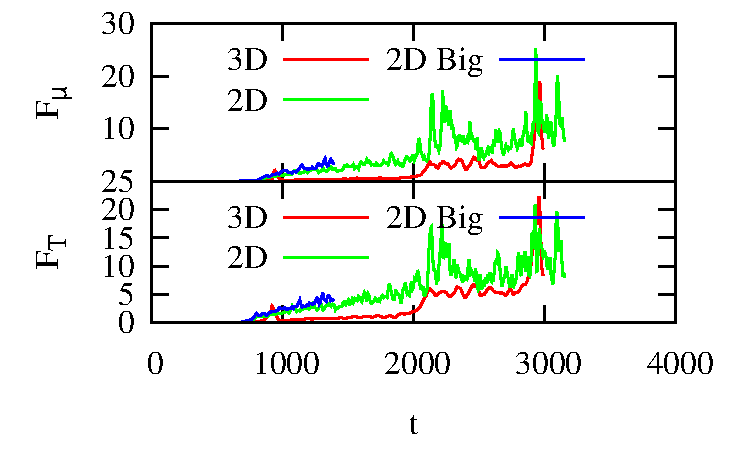
\includegraphics[width=0.35\textwidth]{figs/Pr=0_01_t=0_01_R0-1=1_5.pdf}}}} &
% 	\fbox{\vtop{\null\hbox{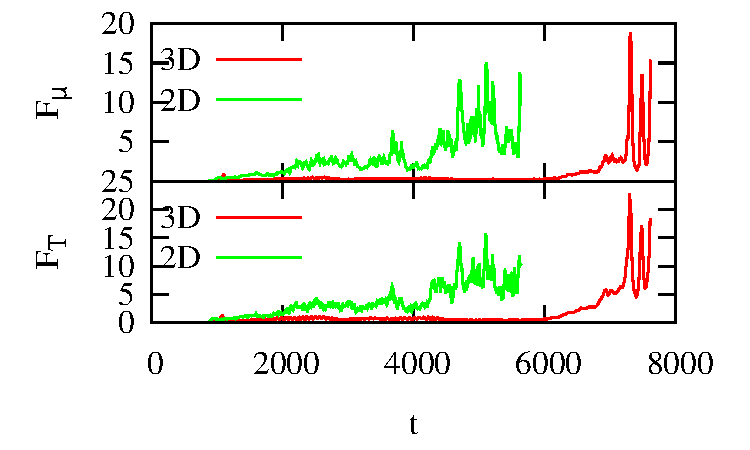
\includegraphics[width=0.35\textwidth]{figs/Pr=0_01_t=0_01_R0-1=2.pdf}}}} \\
% \end{tabular}
% }

% \frame{\frametitle{These simulations show no sign of the strong horizontal shear apparent in the simulations at higher viscosity.}
% \begin{figure}[h]
% 	\centering
% 		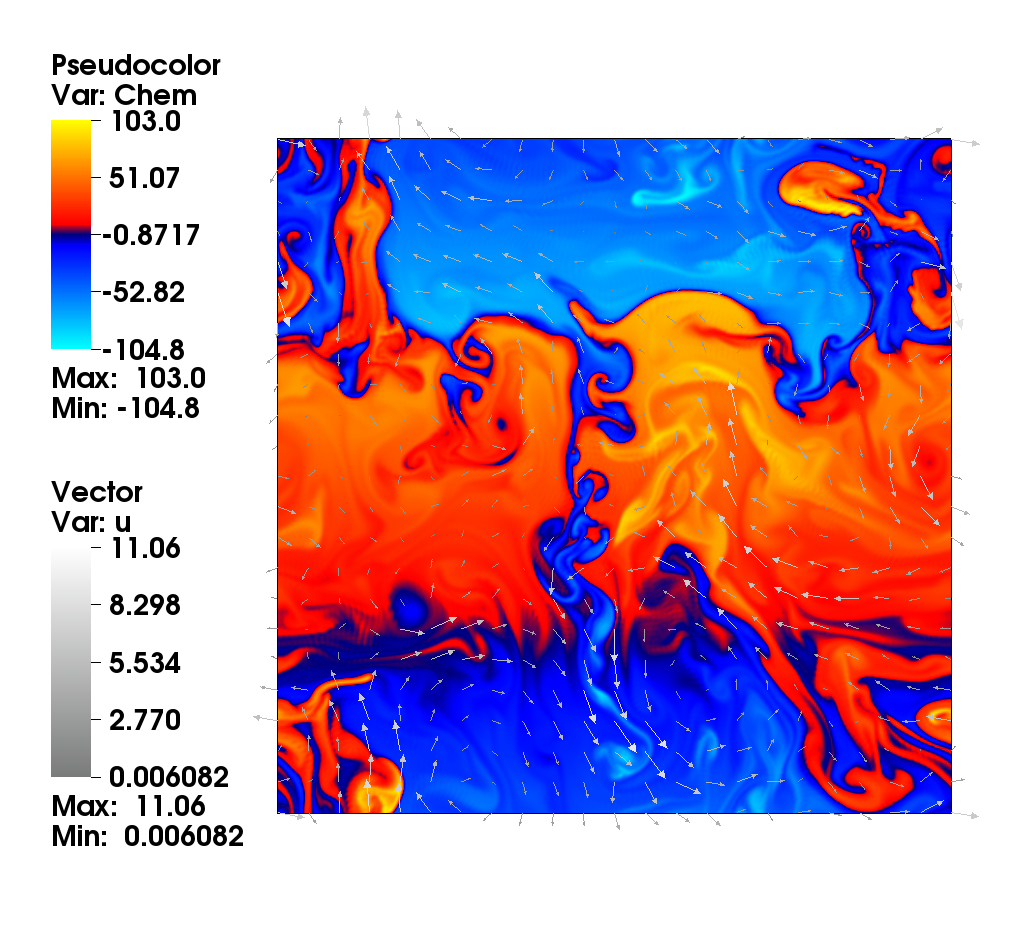
\includegraphics[width=.55\textwidth]{../pngs/sc_layers_0-03_0-03.png}
% 	\caption{$\rm{Pr}=0.03$, $\tau=0.03$, $R_{0}^{-1}=1.5$}
% 	\label{fig:pngs_sc_layers_0-03_0-03}
% \end{figure}
% }

\section{(P)ISCES}

\frame{\tableofcontents[hideothersubsections]}

\frame{\frametitle{Boundary conditions}
\begin{columns}
	\column{125pt}
	\begin{itemize}
		\item Fixed outer vertical boundaries
		\item Periodic horizontal boundaries 
		\item Cross-element boundaries must be continuous and smooth
	\end{itemize}
	\column{175pt}
	\begin{figure}[h]
		\centering
			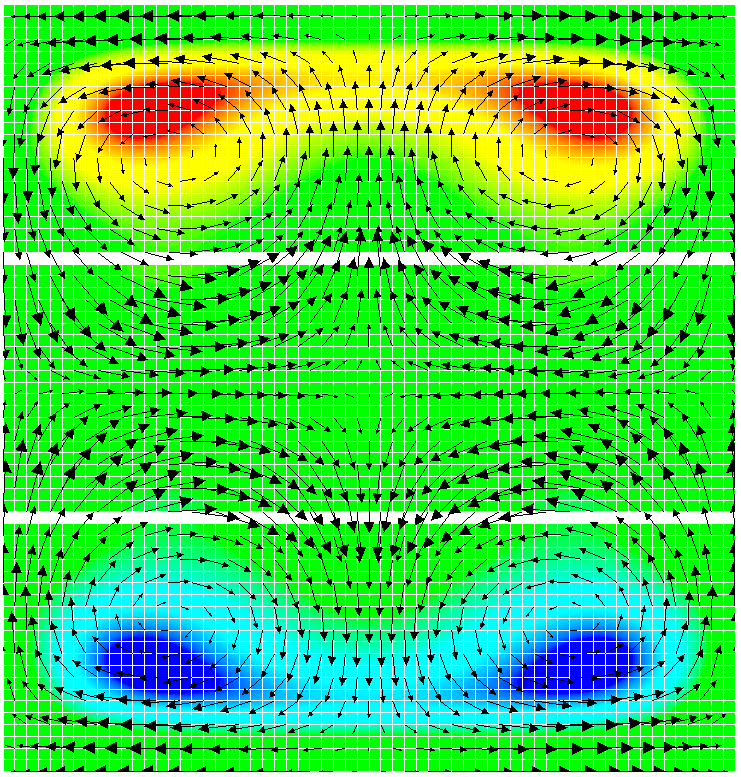
\includegraphics[width=0.8\textwidth]{figs/elements.png}
		\label{fig:figs_elements}
	\end{figure}
\end{columns}}

\subsection{(Pseudo-)Incompressible}

\frame{\frametitle{The code currently constrains the velocity using a predictor-corrector method according to the incompressible velocity constraint \citep{Chorin1997}.}
\begin{align}
	\nabla\cdot\mathbf{u}^{\rm{new}}=&0
\end{align}
Update the velocity according to the momentum equation, ignoring the pressure term.
\begin{align}
	\rho_{0}\frac{D}{Dt}\mathbf{u^{\rm{mid}}}=&\left(-\alpha{T}+\beta\mu\right)\rho_{0}\mathbf{g} + \nu\rho_{0}\nabla^{2}\mathbf{u^{\rm{mid}}}\\
	\frac{\mathbf{u}^{\rm{new}}-\mathbf{\mathbf{u}^{\rm{mid}}}}{\Delta t}=&-\frac{\nabla{p}}{\rho_{0}} \\
	\frac{-\nabla\cdot\mathbf{\mathbf{u}^{\rm{mid}}}}{\Delta t}=&-\nabla\cdot\frac{\nabla{p}}{\rho_{0}}
\end{align}
}

\subsection{Spectral-Chebyshev}

\frame{\frametitle{The code is pseudo-spectral, calculating the non-linear terms in Cartesian space and implicit terms in spectral space.}
\begin{overprint}
	\only<1>{
	\begin{itemize}
		\item Fourier series in the horizontal to enforce periodicity
		\item Chebyshev polynomials in the vertical for fine boundary resolution
	\end{itemize}
	\begin{equation}
		F\left(x,z\right)=\sum_{j=-N_{x}/2}^{N_{x}/2}\sum_{k=0}^{N_{z}}f_{i,j}e^{\frac{2\pi ij\left(x-x_{0}\right)}{L_{x}}}T_{k}\left(\frac{z-z_{0}}{L_{z}/2}\right) 
	\end{equation}
	}
\end{overprint}
}

\subsection{Element Solver}

\frame{\frametitle{The code solves the diffusion implicitly by alternating directions, solving by collocation in the vertical and by spectral method in the horizontal.}
\begin{align}
	\sum_{k}\left(T_{k}\left(\frac{z_{l}-z_{0}}{L_{z}/2}\right)-\kappa\left(z_{l}\right)\frac{\Delta t}{L_{z}^{2}/4} T''_{k}\left(\frac{z_{l}-z_{0}}{L_{z}/2}\right)\right) f_{j,k}^{\rm{new}}=& \nonumber \\
	F_{j}^{\rm{old}}\left(z_{l}\right)+\Delta t RHS_{j}\left(z_{l}\right)&
\end{align}
We can solve equations with $z$-dependent coefficients implicitly
\begin{equation}
	\left(1-\kappa\left(z_{l}\right)\Delta t\left(\frac{2\pi  ij}{L_{x}}\right)^{2}\right)F^{\rm{new}}_{j}\left(z_{l}\right)=F^{\rm{old}}_{j}\left(z_{l}\right)+\Delta t  RHS_{j}\left(z_{l}\right)
\end{equation}
}

\subsubsection{Collocation Matrix Solve}

\frame{\frametitle{The collocation method matches the boundaries of the elements with spectral accuracy; the matrix can be solved as follows (Beaume, private communication).}
\begin{overprint}
	\only<1>{\scalebox{0.7}{$\left(\begin{array}{c c c c c c c}
	A_{0,0} & A_{1,0} & 0 & 0 & \dots & 0 & 0 \\
	A_{0,1} & A_{1,1} & A_{2,1} & 0 & \dots & 0 & 0 \\
	0 & A_{1,2} & A_{2,2} & A_{3,2} & \dots & 0 & 0 \\
	0 & 0 & A_{2,3} & A_{3,3} & \dots & 0 & 0 \\
	\vdots & \vdots & \vdots & \vdots & \ddots & A_{N-2,N-3} & 0 \\
	0 & 0 & 0 & 0 & A_{N-3,N-2} & A_{N-2,N-2} & A_{N-1,N-2} \\
	0 & 0 & 0 & 0 & 0 & A_{N-2,N-1} & A_{N-1,N-1} 
\end{array}\right)
\left(\begin{array}{c}
	X_{0}\\
	X_{1}\\
	X_{2}\\
	X_{3}\\
	\vdots\\
	X_{N-2}\\
	X_{N-1}
\end{array}\right)=
\left(\begin{array}{c}
	B_{0}\\
	B_{1}\\
	B_{2}\\
	B_{3}\\
	\vdots\\
	B_{N-2}\\
	B_{N-1}
\end{array}\right)$}
	}
	\only<2>{\scalebox{0.9}{$\left(\begin{array}{c c c c c | c c c c}
	A_{0,0} & 0 & \dots & \dots &  0 & A_{1,0} & 0 & \dots & 0 \\
	0 & A_{2,2} & \dots & \dots &  0 & A_{1,2} & A_{3,2} & \dots & 0 \\
	\vdots & \vdots & \ddots & \dots & \vdots & \vdots & \ddots & \ddots & \vdots \\
	0 & 0 & \dots & \ddots & 0 & 0 & 0 & \ddots & A_{N-2,N-3} \\
	0 & 0 & \dots & \dots & A_{N-1,N-1} & 0 & 0 & \dots & A_{N-2,N-1} \\
	\hline
	A_{0,1} & A_{2,1} & \dots & 0 & 0 & A_{1,1}  & 0 & \dots & 0 \\
	0 & A_{2,3} & \ddots & 0 & 0 & 0 & A_{3,3} & \dots & 0 \\
	\vdots & \vdots & \ddots & \ddots & \vdots & \vdots & \vdots & \ddots & \vdots \\
	0 & 0 & \dots & A_{N-3,N-2} & A_{N-1,N-2} & 0 & 0 & \dots & A_{N-2,N-2} \\
\end{array}\right)$}}
	\only<3>{
	\begin{align}
	\left(\begin{array}{c c}
		A_{TL} & A_{TR} \\
		A_{BL} & A_{BR}
	\end{array}\right)
	\left(\begin{array}{c}
		X_{L}\\
		X_{R}
	\end{array}\right)=&
	\left(\begin{array}{c}
		B_{T}\\
		B_{B}
	\end{array}\right)\\
		A_{TL}X_{L}+A_{TR}X_{R}=&B_{T}\\
		A_{BL}X_{L}+A_{BL}A_{TL}^{-1}A_{TR}X_{R}=&A_{BL}A_{TL}^{-1}B_{T}\\
	\left(\begin{array}{c c}
			A_{TL} & 0 \\
			0 & A_{BR}-A_{BL}A_{TL}^{-1}A_{TR}
		\end{array}\right)&
		\left(\begin{array}{c}
			X_{L}+A_{TR}X_{R}\\
			X_{R}
		\end{array}\right)=\\
		&\left(\begin{array}{c}
			B_{T}\\
			B_{B}-A_{BL}A_{TL}^{-1}B_{T} 
		\end{array}\right)
		\end{align}
		}
\end{overprint}
}

\subsubsection{Dynamic Boundaries}

\frame{\frametitle{The extents of these elements are dynamic, and can be rezoned using simulated annealing.}
% \begin{overprint}
% 	\only<1>{
% We define $P (E (s), E (s'), T)$, the probability to accept a new state, $s'$, to maximize $E$, given a temperature, $T$, where $P > 0$ even if $E(s') < E(s)$ but that $P (E(s') < E(s)) \rightarrow 0$ as $T \rightarrow 0$.\footnote{Pseudocode from Wikipedia}
% \begin{itemize}
% 	\item Let $s = s_{0}$
% 	\item For $k$ in 0 to $k_{\rm{max}}$:
% 	\begin{itemize}
% 		\item $T =$ temperature ($\frac{k}{k_{\rm{max}}}$)
% 		\item Pick a random neighbor, $s'$ = neighbor ($s$)
% 		\item If $P(E(s), E(s'), T) >$ random(0, 1):
% 		\begin{itemize}
% 			\item $s = s_{\rm{new}}$
% 		\end{itemize}
% 	\end{itemize}
% 	\item Return: $s$
% \end{itemize}}
% \only<2>{
\begin{figure}
	\includemedia[width=\columnwidth,activate=onclick]{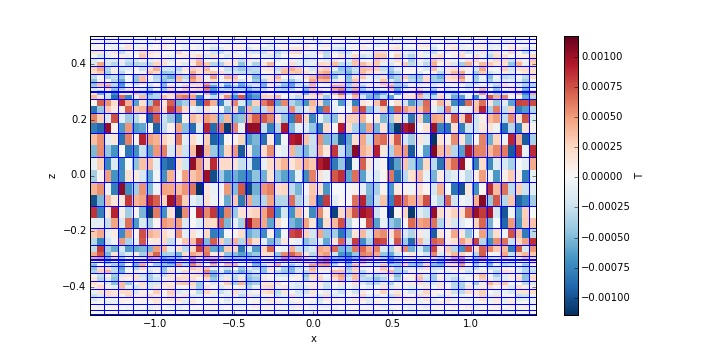
\includegraphics[width=\columnwidth,height=160pt]{out_00.png}}{out.swf}
\end{figure}
% }
% \end{overprint}
}

\subsection{Results}

\frame{\frametitle{To verify the code, we ran the standard Rayleigh B\'enard Convection problem and compared to \citet{Moore1973}.}
\begin{figure}[h]
	\centering
		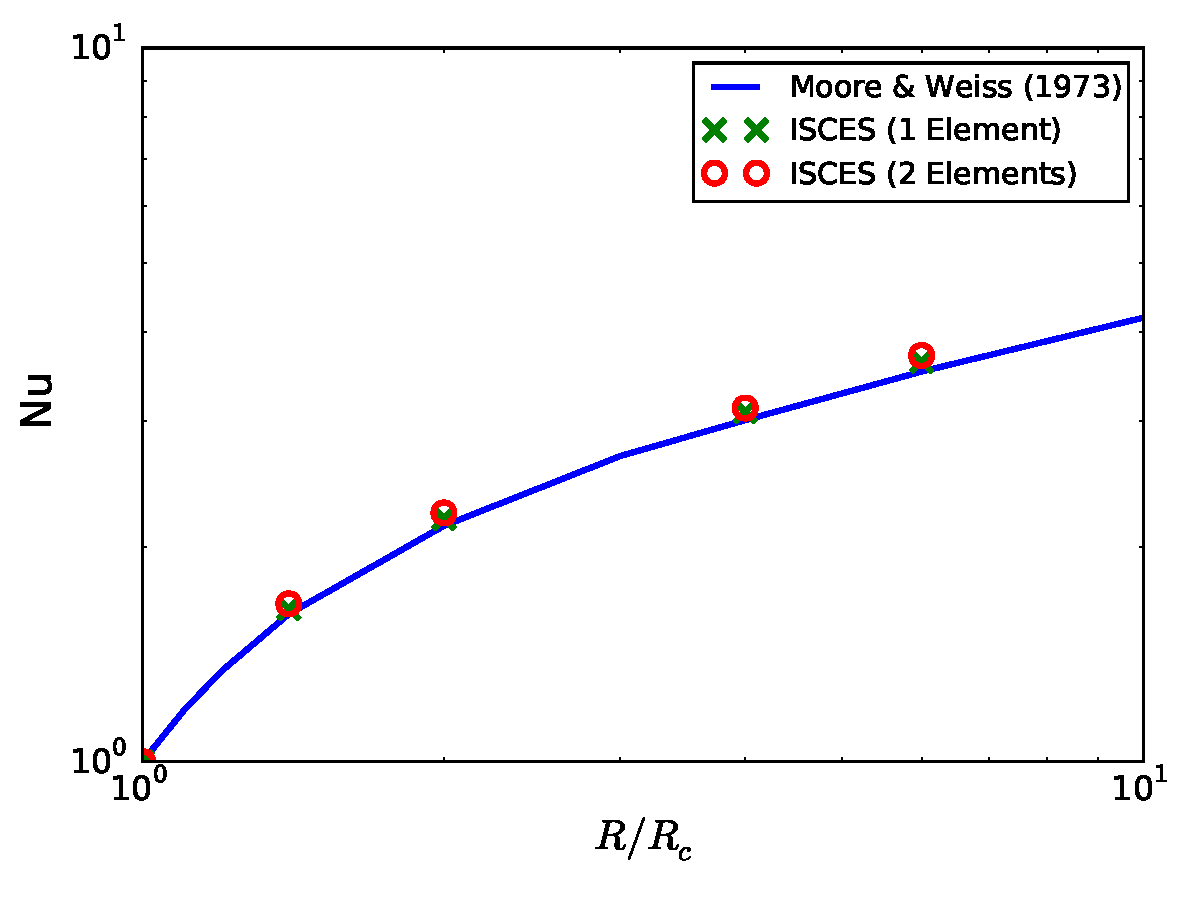
\includegraphics[width=.7\textwidth]{verify.pdf}
	\label{fig:verify}
\end{figure}
}

\frame{\frametitle{We can also compare to the results of the same equations with the same parameters as PADDI.}
\begin{figure}[h]
	\centering
		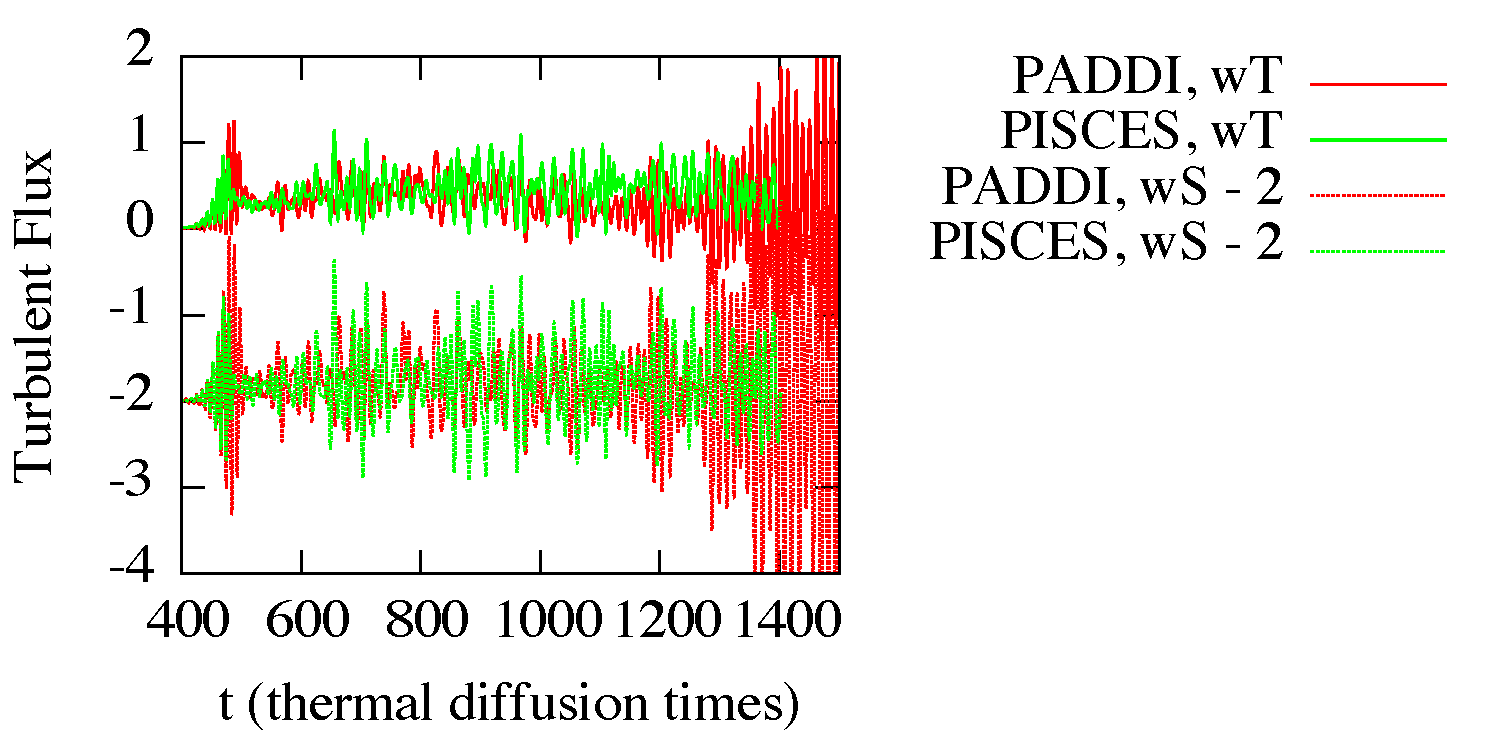
\includegraphics[width=.9\textwidth]{figs/sc_gwave.pdf}
	\caption{The late time behavior is dominated by the boundary conditions, which differ between the codes}
	\label{fig:figs_sc_gwave}
\end{figure}
}

\frame{\frametitle{We are investigating the differences between heating and variable diffusion.}
\begin{figure}[h]
	\centering
		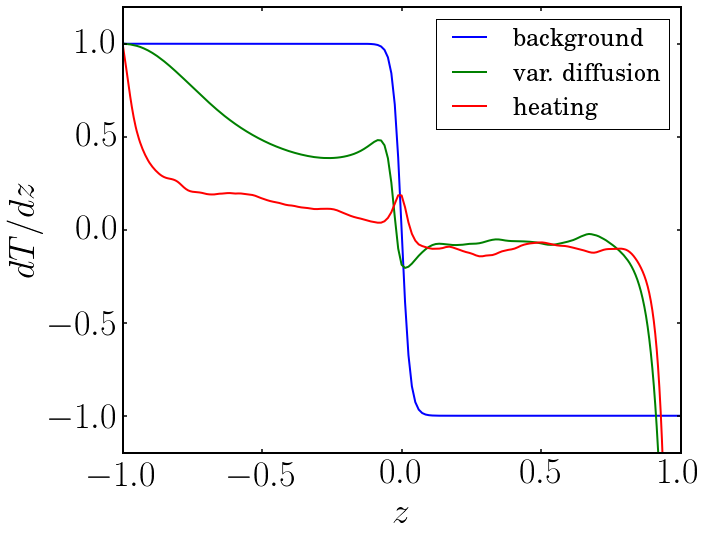
\includegraphics[width=.7\textwidth]{figs/variable_vs_heat.png}
	\label{fig:var_vs_heat}
\end{figure}
}

\section{Future}

\frame{\tableofcontents[hideothersubsections]}

% \subsection{Layered Semi-Convection}

% \frame{\frametitle{Future Code Development}
% \begin{itemize}
% 	\item Implement nonlinear diffusion (working in 1D) in 2D
% 	\begin{itemize}
% 		\item Examine layer properties with $\mu$-dependent diffusion
% 	\end{itemize}
% 	\item Upgrade from Boussinesq to Pseudo-Incompressible
% 	\begin{itemize}
% 		\item Determine layer height across density scale heights
% 	\end{itemize}
% 	\item Update KEPLER and MESA with layer height
% \end{itemize}}

\subsection{Additional Slides}

\frame{\tableofcontents[hideothersubsections]}

\subsubsection{Pseudo-Incompressibility}

\frame{\frametitle{Governing equations}
\begin{overprint}
	\only<1>{\bf Fully Compressible}
	\only<2>{\bf Incompressible, Current Equations}
	\only<3>{\bf Pseudo-Incompressible}
	% \only<4>{\bf Pseudo-Incompressible, Energy Conserving (Wood, private communication)}
	\only<1>{
	\begin{align}
		\rho\frac{D}{D{t}}{\mathbf{u}} =& -\nabla p + \rho \mathbf{g} + \nabla\cdot\mathbf{\Pi} \\
		\frac{D}{D{t}}\rho =& -\rho\nabla\cdot\mathbf{u} \\
		\rho{T}\frac{D}{D{t}}{s} =& \nabla\vect{u}:\vect{\Pi} + \sum_{i}\mu_{i}\nabla\cdot\vect{C}_{i} - \nabla\cdot{\vect{H}} \\
		\rho\frac{D}{D{t}}{\xi_{i}}=&-\nabla\cdot\vect{C}_{i}
	\end{align}}
	\only<2>{
	\begin{align}
		\rho_{0}\frac{D}{D{t}}{\mathbf{u}} =& -\nabla p + \left(-\alpha{T}+\beta\mu\right)\rho_{0}\mathbf{g} + \nu\rho_{0}\nabla^{2}\mathbf{u} \\
		\nabla\cdot\mathbf{u} =& 0 \\
		\frac{D}{D{t}}{T} + w\frac{d}{dz}T_{0} =& \kappa_T \nabla^{2}T \\
		\frac{D}{D{t}}{\xi_{i}} + w\frac{d}{dz}\xi_{i,0}=& \kappa_{i}\nabla^{2}\xi_{i}
	\end{align}}
	\only<3>{
	\begin{align}
		\rho\frac{D}{D{t}}\mathbf{u}=&-\nabla\left(p_{0}+p_{1}\right)+\frac{p_{1}}{\rho}\left(\frac{\partial p}{\partial \rho}\right)^{-1}\nabla p_{0} -\rho\nabla\Phi+\nabla\cdot\mathbf{\Pi}\\
		p_{0}\left(z\right)=&p\left(\rho,s,\xi_{1},\xi_{2},\dots\right)\\
		\frac{D}{D{t}}\rho =& -\rho\nabla\cdot\mathbf{u} \\
		\rho{T}\frac{D}{D{t}}{s} =& \nabla\mathbf{u}:\mathbf{\Pi} + \sum_{i}\mu_{i}\nabla\cdot\mathbf{C}_{i} - \nabla\cdot{\mathbf{H}}\\
		\rho\frac{D}{D{t}}\xi_{i}=&-\nabla\cdot\mathbf{C}_{i}, 
		% \only<4>{\left(T,\mu_{i}\right)\equiv\left(\frac{\partial e}{\partial s},\frac{\partial e}{\partial \xi_{i}}\right)+p_{1}\frac{\partial{\left(\frac{\partial e}{\partial s},\frac{\partial e}{\partial \xi_{i}}\right)}/\partial{\rho}}{\partial{p}/\partial{\rho}}}
	\end{align}}
\end{overprint}
}

\frame{\frametitle{Incompressible Non-Dimensionalization}
	\begin{align}
		\frac{D}{D{t}}{\mathbf{u}} =& -\nabla p + \frac{-\mathrm{Ra}_{T}T+\mathrm{Ra}_{\mu}\mu}{\mathrm{Pr}} + \nabla^{2}\mathbf{u} \\
		\nabla\cdot\mathbf{u} =& 0 \\
		\frac{D}{D{t}}{T} =& \nabla\cdot\left(\mathrm{Pr}^{-1}+\frac{\kappa_{T,1}}{\nu}\left(z\right)\right) \nabla T \\
		\frac{D}{D{t}}{\xi_{i}} =& \frac{\tau}{\mathrm{Pr}}\nabla^{2}\xi_{i}
	\end{align}
}

\frame{\frametitle{To solve these equations, we choose the equation of state of an ideal mixture.}
	\begin{align}
		\rho\frac{D}{D{t}}\mathbf{u}=&-\nabla\left(p_{0}+p_{1}\right)+\frac{p_{1}}{\gamma p_{0}}\nabla p_{0} -\rho\nabla\Phi+\nabla\cdot\mathbf{\Pi}\\
		p_{0}\left(z\right)=&\frac{k\rho\tilde{T}}{\overline{m}}\\
		\frac{D}{D{t}}\rho =& -\rho\nabla\cdot\mathbf{u} \\
		\rho{T}\frac{D}{D{t}}{s} =& \nabla\mathbf{u}:\mathbf{\Pi} + \sum_{i}\mu_{i}\nabla\cdot\mathbf{C}_{i} - \nabla\cdot{\mathbf{H}}\\
		\rho\frac{D}{D{t}}\xi_{i}=&-\nabla\cdot\mathbf{C}_{i}, \left(T,\mu_{i}\right)\equiv\frac{c_{p}p_{0}+kp_{1}}{c_{p}p_{0}}\left(\tilde{T},\tilde{\mu_{i}}\right)
	\end{align}
}

\frame{\frametitle{We can simplify this by expressing the entropy equation as a temperature equation.}
\begin{overprint}
	\only<1>{
		\begin{equation}
			\frac{D}{Dt}T=\frac{\partial T}{\partial \rho}\frac{D}{Dt}\rho + \frac{\partial T}{\partial s}\frac{D}{Dt}s + \frac{\partial T}{\partial \xi_{i}}\frac{D}{Dt}\xi_{i}.
		\end{equation}
		We can use the remainder of the governing equations and the equation of state to get the full equation.
	}
	\only<2>{
		\begin{equation}
			\rho\frac{D}{Dt}T=-\left(\gamma - 1\right)\rho T\nabla\cdot{u} + \left(\gamma - 1\right)\frac{\overline{m}}{k}\left(\nabla\vect{u}:\vect{\Pi}-\nabla\cdot{\vect{H}}\right).
		\end{equation}
	}
\end{overprint}
}

\frame{\frametitle{Governing Equations}
	\begin{align}
		p_{0} &= \frac{\rho T}{\overline{m}} \\
		\rho\frac{D}{Dt}\vect{u} &= -\nabla\left(p_{0} + p_{1}\right) + \frac{p_{1}}{\gamma p_{0}}\nabla{p_{0}} - \rho \hat{y} + \nabla \cdot \vect{\Pi} \\
		\rho\frac{D}{Dt}\xi &= \nabla \cdot \rho \tau \nabla \xi \\
		\frac{1}{\gamma - 1}\rho\frac{D}{Dt} T &= -\rho T \nabla \cdot \vect{u} + \overline{m}\left(\nabla\vect{u}:\vect{\Pi} + \nabla\cdot \frac{\rho}{\overline{m}}\nabla{T}\right)\left(1 + Q\right) \\
		\nabla\cdot{p_{0}^{\frac{1}{\gamma}}} &= \frac{\gamma - 1}{\gamma}p_{0}^{\frac{1}{\gamma}-1}\left(\nabla\vect{u}:\vect{\Pi}-\nabla\cdot \frac{\rho}{\overline{m}}\nabla{T}\right)\left(1 + Q\right) \\
		\Pi_{ij} &= \rho \mathrm{Pr}\left(\frac{\partial u_{i}}{\partial x_{j}} + \frac{\partial u_{j}}{\partial x_{i}} - \frac{2}{3}\delta_{ij}\nabla\cdot{\vect{u}}\right)
	\end{align}
}

\subsubsection{Two-Component Ideal Mixture}

\frame{\frametitle{Derivation of the Equation of State for a two-component mixture.}
\begin{overprint}
	\only<1>{
	Start with the EOS for an ideal gas:
	\begin{align}
		e_{i}\left(\rho_{i},s_{i}\right)=&\frac{c_{V}}{m_{i}}\left(\frac{\rho_{i}}{m_{i}}\phi_{i} e^{\frac{m_{i}s_{i}}{k}}\right)^{\frac{k}{c_{V}}}
	\end{align}
	Each component of the gas must follow this, and the total energy is $\overline{m}e=m_{1}e_{1}+m_{2}e_{2}$.
	}
	\only<2>{
	Note the entropy of the mixture is defined as $\overline{m}s=m_{1}\xi_{1}s_{1}+_{2}\xi_{2}s_{2}-k\xi_{1}\ln{\xi_{1}}-k\xi_{2}\ln{\xi_{2}}$.
	We assume the gases are thermally coupled:
	\begin{align}
		T=&\left(\frac{\rho\xi_{1}\phi_{1}}{\overline{m}}e^{\frac{m_{1}s_{1}}{k}}\right)^{\frac{k}{c_{v}}}=\left(\frac{\rho\xi_{2}\phi_{2}}{\overline{m}}e^{\frac{m_{2}s_{2}}{k}}\right)^{\frac{k}{c_{v}}}\\
		e^{\frac{m_{1}s_{1}}{k}}=&\left(\frac{\xi_{2}\phi_{2}}{\xi_{1}\phi_{1}}\right)^{\xi_{2}}e^{\frac{\overline{m}s}{k}+\xi_{1}\ln{\xi_{1}}+\xi_{2}\ln{\xi_{2}}}
	\end{align}
	And likewise for $s_{2}$
	}
	\only<3>{
	Thus, the total energy is
\begin{align}
	e_{1}\left(\rho,s,\xi_{1},\xi_{2}\right)&=c_{V}\left(\frac{\rho\xi_{1}\phi_{1}}{m_{1}}\left[\frac{\xi_{2}\phi_{2}}{\xi_{1}\phi{1}}\right]^{\xi_{2}} e^{\frac{\overline{m}s}{k}+\xi_{1}\ln{\xi_{1}}+\xi_{2}\ln{\xi_{2}}}\right)^{\frac{k}{c_{V}}},\\
	e_{2}\left(\rho,s,\xi_{1},\xi_{2}\right)&=c_{V}\left(\frac{\rho\xi_{2}\phi_{2}}{m_{2}}\left[\frac{\xi_{1}\phi_{1}}{\xi_{2}\phi{2}}\right]^{\xi_{1}} e^{\frac{\overline{m}s}{k}+\xi_{1}\ln{\xi_{1}}+\xi_{2}\ln{\xi_{2}}}\right)^{\frac{k}{c_{V}}},\\
	\overline{m} e\left(\rho,s,\xi_{1}\right)&=\sum_{i} m_{i} \xi_{i} e_{i}\left(\rho,s,\xi_{1},1-\xi_{1}\right).
\end{align}
	}
	\only<4>{
	\begin{tabular}{|r | c | c | c |}
		\hline
		 & & $\frac{\partial}{\partial \rho}$ & $\frac{\partial/\partial \rho}{\partial p / \partial \rho}$ \\ \hline
		$p$ & $\frac{k}{c_{v}}\rho e$ & $\frac{c_{p}}{c_{v}}\frac{p}{\rho}$ & 1 \\ \hline
		$T$ & $\frac{e}{c_{v}}$ & $\frac{kT}{c_{v}\rho}$ & $\frac{kT}{c_{p}p}$ \\ \hline
		$\mu_{1}$ & $\frac{\frac{1}{\xi_{1}}\left(m_{2}-\overline{m}\right)\left(c_{p}-\overline{m}s\right)+k\ln{\frac{\phi_{1}}{\phi_{2}}}}{c_{v}}e$ & $\frac{k\mu_{1}}{c_{v}\rho}$ & $\frac{k\mu_{1}}{c_{p}p}$ \\ \hline
	\end{tabular}
	}
\end{overprint}
}

\begingroup
\renewcommand{\section}[2]{}%
%\renewcommand{\chapter}[2]{}% for other classes
\bibliography{Fluids,Nucleosynthesis,Evolution}
\endgroup

\end{document}